\documentclass[1p]{elsarticle_modified}
%\bibliographystyle{elsarticle-num}

%\usepackage[colorlinks]{hyperref}
%\usepackage{abbrmath_seonhwa} %\Abb, \Ascr, \Acal ,\Abf, \Afrak
\usepackage{amsfonts}
\usepackage{amssymb}
\usepackage{amsmath}
\usepackage{amsthm}
\usepackage{scalefnt}
\usepackage{amsbsy}
\usepackage{kotex}
\usepackage{caption}
\usepackage{subfig}
\usepackage{color}
\usepackage{graphicx}
\usepackage{xcolor} %% white, black, red, green, blue, cyan, magenta, yellow
\usepackage{float}
\usepackage{setspace}
\usepackage{hyperref}

\usepackage{tikz}
\usetikzlibrary{arrows}

\usepackage{multirow}
\usepackage{array} % fixed length table
\usepackage{hhline}

%%%%%%%%%%%%%%%%%%%%%
\makeatletter
\renewcommand*\env@matrix[1][\arraystretch]{%
	\edef\arraystretch{#1}%
	\hskip -\arraycolsep
	\let\@ifnextchar\new@ifnextchar
	\array{*\c@MaxMatrixCols c}}
\makeatother %https://tex.stackexchange.com/questions/14071/how-can-i-increase-the-line-spacing-in-a-matrix
%%%%%%%%%%%%%%%

\usepackage[normalem]{ulem}

\newcommand{\msout}[1]{\ifmmode\text{\sout{\ensuremath{#1}}}\else\sout{#1}\fi}
%SOURCE: \msout is \stkout macro in https://tex.stackexchange.com/questions/20609/strikeout-in-math-mode

\newcommand{\cancel}[1]{
	\ifmmode
	{\color{red}\msout{#1}}
	\else
	{\color{red}\sout{#1}}
	\fi
}

\newcommand{\add}[1]{
	{\color{blue}\uwave{#1}}
}

\newcommand{\replace}[2]{
	\ifmmode
	{\color{red}\msout{#1}}{\color{blue}\uwave{#2}}
	\else
	{\color{red}\sout{#1}}{\color{blue}\uwave{#2}}
	\fi
}

\newcommand{\Sol}{\mathcal{S}} %segment
\newcommand{\D}{D} %diagram
\newcommand{\A}{\mathcal{A}} %arc


%%%%%%%%%%%%%%%%%%%%%%%%%%%%%5 test

\def\sl{\operatorname{\textup{SL}}(2,\Cbb)}
\def\psl{\operatorname{\textup{PSL}}(2,\Cbb)}
\def\quan{\mkern 1mu \triangleright \mkern 1mu}

\theoremstyle{definition}
\newtheorem{thm}{Theorem}[section]
\newtheorem{prop}[thm]{Proposition}
\newtheorem{lem}[thm]{Lemma}
\newtheorem{ques}[thm]{Question}
\newtheorem{cor}[thm]{Corollary}
\newtheorem{defn}[thm]{Definition}
\newtheorem{exam}[thm]{Example}
\newtheorem{rmk}[thm]{Remark}
\newtheorem{alg}[thm]{Algorithm}

\newcommand{\I}{\sqrt{-1}}
\begin{document}

%\begin{frontmatter}
%
%\title{Boundary parabolic representations of knots up to 8 crossings}
%
%%% Group authors per affiliation:
%\author{Yunhi Cho} 
%\address{Department of Mathematics, University of Seoul, Seoul, Korea}
%\ead{yhcho@uos.ac.kr}
%
%
%\author{Seonhwa Kim} %\fnref{s_kim}}
%\address{Center for Geometry and Physics, Institute for Basic Science, Pohang, 37673, Korea}
%\ead{ryeona17@ibs.re.kr}
%
%\author{Hyuk Kim}
%\address{Department of Mathematical Sciences, Seoul National University, Seoul 08826, Korea}
%\ead{hyukkim@snu.ac.kr}
%
%\author{Seokbeom Yoon}
%\address{Department of Mathematical Sciences, Seoul National University, Seoul, 08826,  Korea}
%\ead{sbyoon15@snu.ac.kr}
%
%\begin{abstract}
%We find all boundary parabolic representation of knots up to 8 crossings.
%
%\end{abstract}
%\begin{keyword}
%    \MSC[2010] 57M25 
%\end{keyword}
%
%\end{frontmatter}

%\linenumbers
%\tableofcontents
%
\newcommand\colored[1]{\textcolor{white}{\rule[-0.35ex]{0.8em}{1.4ex}}\kern-0.8em\color{red} #1}%
%\newcommand\colored[1]{\textcolor{white}{ #1}\kern-2.17ex	\textcolor{white}{ #1}\kern-1.81ex	\textcolor{white}{ #1}\kern-2.15ex\color{red}#1	}

{\Large $\underline{12a_{1025}~(K12a_{1025})}$}

\setlength{\tabcolsep}{10pt}
\renewcommand{\arraystretch}{1.6}
\vspace{1cm}\begin{tabular}{m{100pt}>{\centering\arraybackslash}m{274pt}}
\multirow{5}{120pt}{
	\centering
	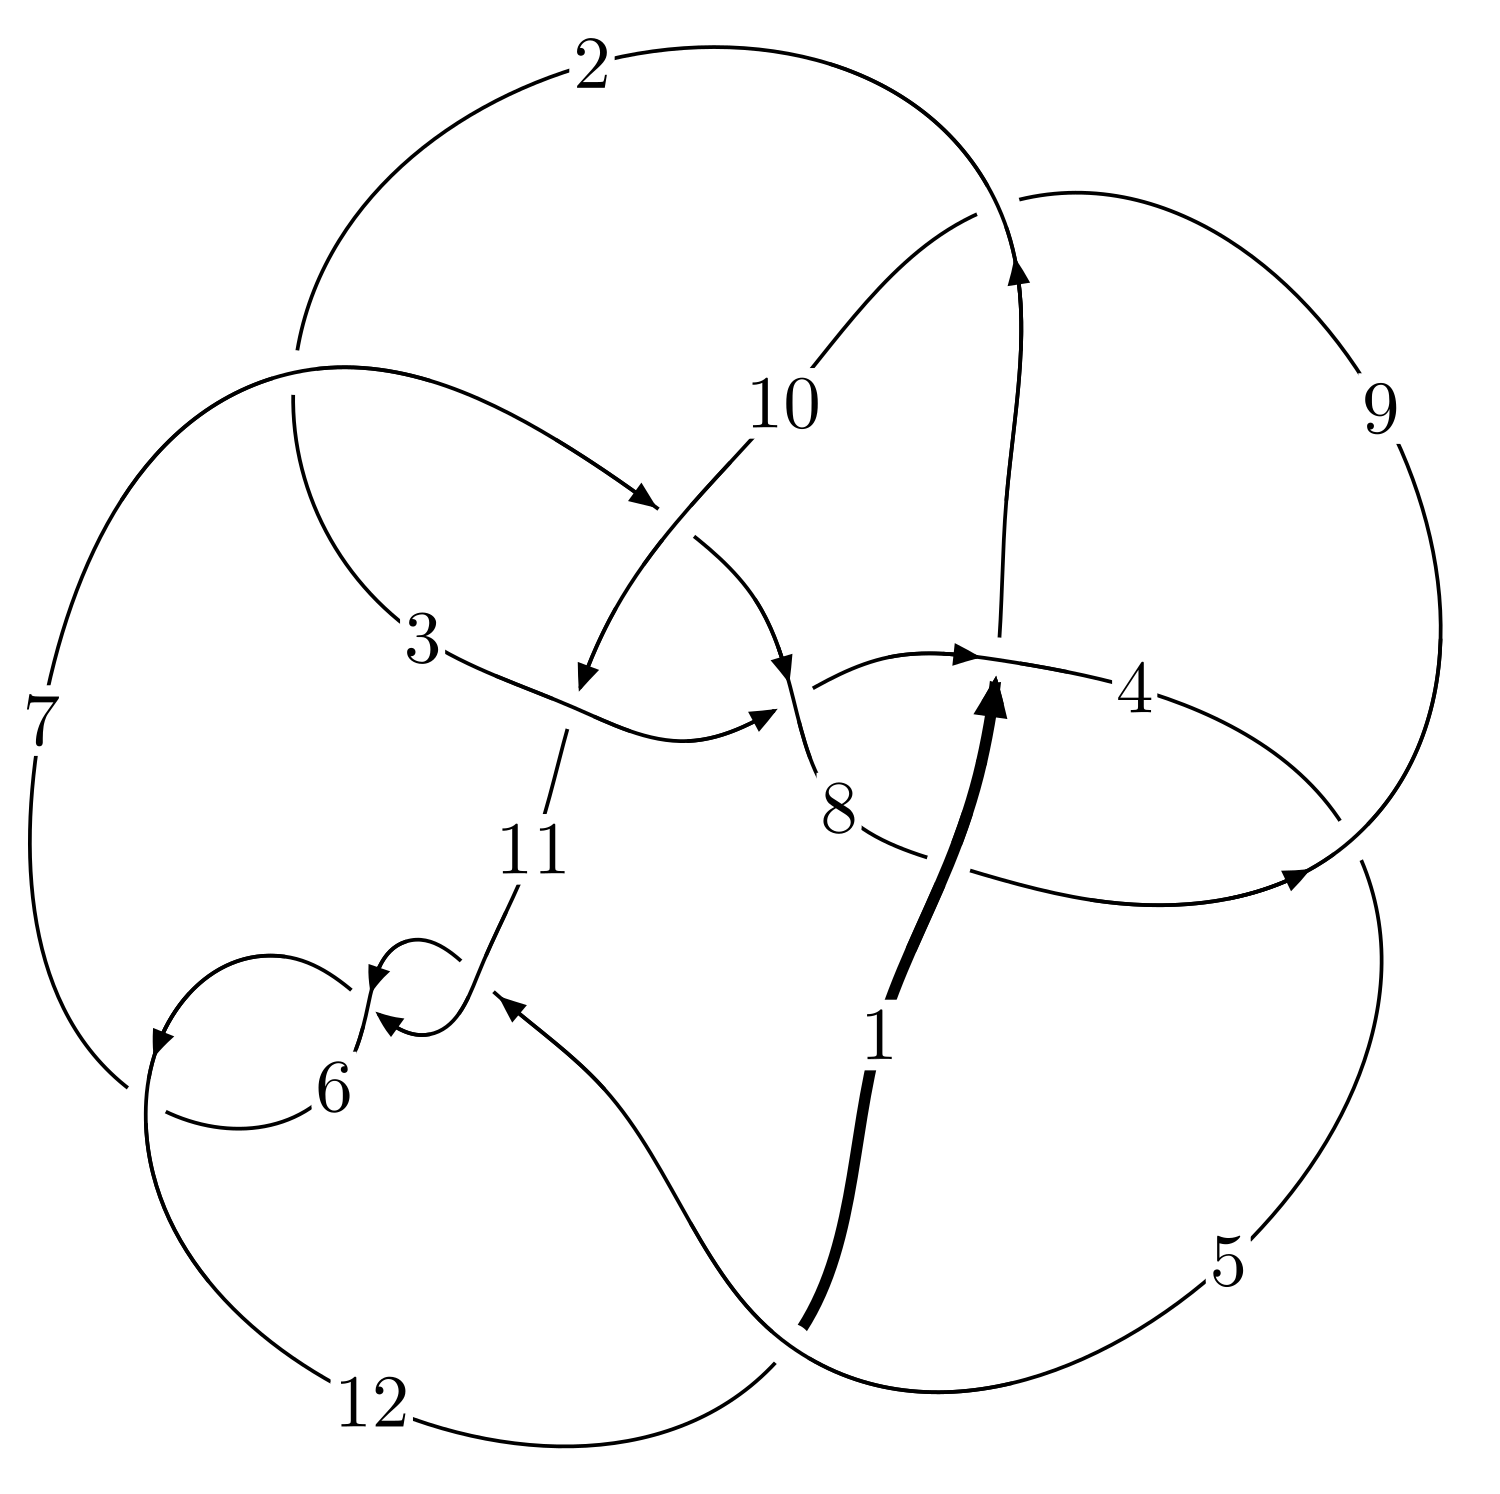
\includegraphics[width=112pt]{../../../GIT/diagram.site/Diagrams/png/1826_12a_1025.png}\\
\ \ \ A knot diagram\footnotemark}&
\allowdisplaybreaks
\textbf{Linearized knot diagam} \\
\cline{2-2}
 &
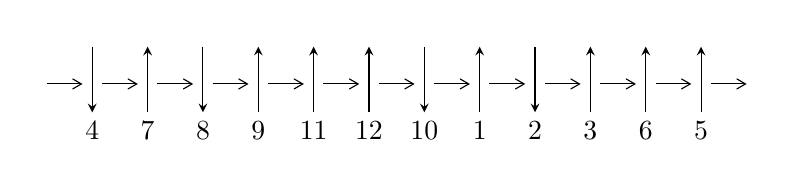
\begin{tikzpicture}[x=20pt, y=17pt]
	% nodes
	\node (C0) at (0, 0) {};
	\node (C1) at (1, 0) {};
	\node (C1U) at (1, +1) {};
	\node (C1D) at (1, -1) {4};

	\node (C2) at (2, 0) {};
	\node (C2U) at (2, +1) {};
	\node (C2D) at (2, -1) {7};

	\node (C3) at (3, 0) {};
	\node (C3U) at (3, +1) {};
	\node (C3D) at (3, -1) {8};

	\node (C4) at (4, 0) {};
	\node (C4U) at (4, +1) {};
	\node (C4D) at (4, -1) {9};

	\node (C5) at (5, 0) {};
	\node (C5U) at (5, +1) {};
	\node (C5D) at (5, -1) {11};

	\node (C6) at (6, 0) {};
	\node (C6U) at (6, +1) {};
	\node (C6D) at (6, -1) {12};

	\node (C7) at (7, 0) {};
	\node (C7U) at (7, +1) {};
	\node (C7D) at (7, -1) {10};

	\node (C8) at (8, 0) {};
	\node (C8U) at (8, +1) {};
	\node (C8D) at (8, -1) {1};

	\node (C9) at (9, 0) {};
	\node (C9U) at (9, +1) {};
	\node (C9D) at (9, -1) {2};

	\node (C10) at (10, 0) {};
	\node (C10U) at (10, +1) {};
	\node (C10D) at (10, -1) {3};

	\node (C11) at (11, 0) {};
	\node (C11U) at (11, +1) {};
	\node (C11D) at (11, -1) {6};

	\node (C12) at (12, 0) {};
	\node (C12U) at (12, +1) {};
	\node (C12D) at (12, -1) {5};
	\node (C13) at (13, 0) {};

	% arrows
	\draw[->,>={angle 60}]
	(C0) edge (C1) (C1) edge (C2) (C2) edge (C3) (C3) edge (C4) (C4) edge (C5) (C5) edge (C6) (C6) edge (C7) (C7) edge (C8) (C8) edge (C9) (C9) edge (C10) (C10) edge (C11) (C11) edge (C12) (C12) edge (C13) ;	\draw[->,>=stealth]
	(C1U) edge (C1D) (C2D) edge (C2U) (C3U) edge (C3D) (C4D) edge (C4U) (C5D) edge (C5U) (C6D) edge (C6U) (C7U) edge (C7D) (C8D) edge (C8U) (C9U) edge (C9D) (C10D) edge (C10U) (C11D) edge (C11U) (C12D) edge (C12U) ;
	\end{tikzpicture} \\
\hhline{~~} \\& 
\textbf{Solving Sequence} \\ \cline{2-2} 
 &
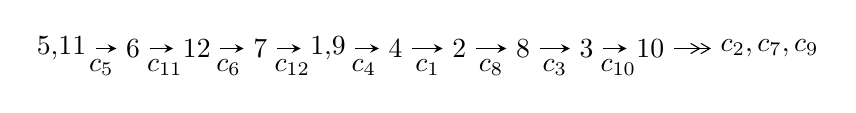
\begin{tikzpicture}[x=23pt, y=7pt]
	% node
	\node (A0) at (-1/8, 0) {5,11};
	\node (A1) at (1, 0) {6};
	\node (A2) at (2, 0) {12};
	\node (A3) at (3, 0) {7};
	\node (A4) at (65/16, 0) {1,9};
	\node (A5) at (41/8, 0) {4};
	\node (A6) at (49/8, 0) {2};
	\node (A7) at (57/8, 0) {8};
	\node (A8) at (65/8, 0) {3};
	\node (A9) at (73/8, 0) {10};
	\node (C1) at (1/2, -1) {$c_{5}$};
	\node (C2) at (3/2, -1) {$c_{11}$};
	\node (C3) at (5/2, -1) {$c_{6}$};
	\node (C4) at (7/2, -1) {$c_{12}$};
	\node (C5) at (37/8, -1) {$c_{4}$};
	\node (C6) at (45/8, -1) {$c_{1}$};
	\node (C7) at (53/8, -1) {$c_{8}$};
	\node (C8) at (61/8, -1) {$c_{3}$};
	\node (C9) at (69/8, -1) {$c_{10}$};
	\node (A10) at (11, 0) {$c_{2},c_{7},c_{9}$};

	% edge
	\draw[->,>=stealth]	
	(A0) edge (A1) (A1) edge (A2) (A2) edge (A3) (A3) edge (A4) (A4) edge (A5) (A5) edge (A6) (A6) edge (A7) (A7) edge (A8) (A8) edge (A9) ;
	\draw[->>,>={angle 60}]	
	(A9) edge (A10);
\end{tikzpicture} \\ 

\end{tabular} \\

\footnotetext{
The image of knot diagram is generated by the software ``\textbf{Draw programme}" developed by Andrew Bartholomew(\url{http://www.layer8.co.uk/maths/draw/index.htm\#Running-draw}), where we modified some parts for our purpose(\url{https://github.com/CATsTAILs/LinksPainter}).
}\phantom \\ \newline 
\centering \textbf{Ideals for irreducible components\footnotemark of $X_{\text{par}}$} 
 
\begin{align*}
I^u_{1}&=\langle 
-8 u^{18}-37 u^{17}+\cdots+2 b+46,\;33 u^{18}+154 u^{17}+\cdots+8 a-196,\;u^{19}+6 u^{18}+\cdots+4 u-8\rangle \\
I^u_{2}&=\langle 
-3 u^{10} a-7 u^9 a+3 u^8 a+8 u^7 a-13 u^6 a-6 u^5 a+8 u^4 a-18 u^3 a-6 u^2 a+9 a u+b-8 a,\\
\phantom{I^u_{2}}&\phantom{= \langle  }-4 u^9 a-7 u^{10}+\cdots+4 a-18,\;u^{11}+4 u^{10}+3 u^9-4 u^8+9 u^6+u^5+2 u^4+12 u^3+u^2-2 u+4\rangle \\
I^u_{3}&=\langle 
19502 u^7 a^3-21027 u^7 a^2+\cdots-98205 a+12679,\;2 u^7 a^3-3 u^7 a^2+\cdots-2 a+5,\\
\phantom{I^u_{3}}&\phantom{= \langle  }u^8- u^7-3 u^6+2 u^5+3 u^4-2 u-1\rangle \\
I^u_{4}&=\langle 
-7.80310\times10^{46} a^{7} u^{7}+1.01169\times10^{47} a^{6} u^{7}+\cdots+1.16866\times10^{48} a+5.76531\times10^{47},\\
\phantom{I^u_{4}}&\phantom{= \langle  }-2 a^7 u^7-10 u^7 a^6+\cdots+388 a-283,\;u^8- u^7-3 u^6+2 u^5+3 u^4-2 u-1\rangle \\
I^u_{5}&=\langle 
-3 u^{31}-13 u^{30}+\cdots+2 b-305,\;631 u^{31}+546 u^{30}+\cdots+78 a+12324,\;u^{32}-17 u^{30}+\cdots+17 u^2-39\rangle \\
I^u_{6}&=\langle 
- u^7+3 u^5-2 u^3+b- u,\;u^5-2 u^3+a+u,\;u^8+u^7-3 u^6-2 u^5+3 u^4+2 u-1\rangle \\
I^u_{7}&=\langle 
- u^7 a+2 u^6 a-2 u^7+2 u^5 a+2 u^6-4 u^4 a+5 u^5- u^3 a-4 u^4+u^2 a-3 u^3+b+2 a- u+3,\\
\phantom{I^u_{7}}&\phantom{= \langle  }-2 u^7 a+2 u^6 a- u^7+5 u^5 a-4 u^4 a+2 u^5-4 u^3 a+3 u^4+2 u^2 a+a^2- a u-5 u^2+2 a-3 u+2,\\
\phantom{I^u_{7}}&\phantom{= \langle  }u^8- u^7-3 u^6+2 u^5+3 u^4-2 u-1\rangle \\
\\
I^v_{1}&=\langle 
a,\;b^2+b+1,\;v+1\rangle \\
\end{align*}
\raggedright * 8 irreducible components of $\dim_{\mathbb{C}}=0$, with total 195 representations.\\
\footnotetext{All coefficients of polynomials are rational numbers. But the coefficients are sometimes approximated in decimal forms when there is not enough margin.}
\newpage
\renewcommand{\arraystretch}{1}
\centering \section*{I. $I^u_{1}= \langle -8 u^{18}-37 u^{17}+\cdots+2 b+46,\;33 u^{18}+154 u^{17}+\cdots+8 a-196,\;u^{19}+6 u^{18}+\cdots+4 u-8 \rangle$}
\flushleft \textbf{(i) Arc colorings}\\
\begin{tabular}{m{7pt} m{180pt} m{7pt} m{180pt} }
\flushright $a_{5}=$&$\begin{pmatrix}1\\0\end{pmatrix}$ \\
\flushright $a_{11}=$&$\begin{pmatrix}0\\u\end{pmatrix}$ \\
\flushright $a_{6}=$&$\begin{pmatrix}1\\- u^2\end{pmatrix}$ \\
\flushright $a_{12}=$&$\begin{pmatrix}u\\- u^3+u\end{pmatrix}$ \\
\flushright $a_{7}=$&$\begin{pmatrix}- u^2+1\\u^4-2 u^2\end{pmatrix}$ \\
\flushright $a_{1}=$&$\begin{pmatrix}- u^3+2 u\\- u^3+u\end{pmatrix}$ \\
\flushright $a_{9}=$&$\begin{pmatrix}-\frac{33}{8} u^{18}-\frac{77}{4} u^{17}+\cdots-31 u+\frac{49}{2}\\4 u^{18}+\frac{37}{2} u^{17}+\cdots+29 u-23\end{pmatrix}$ \\
\flushright $a_{4}=$&$\begin{pmatrix}-\frac{13}{8} u^{18}-8 u^{17}+\cdots-\frac{23}{2} u+\frac{21}{2}\\-\frac{21}{4} u^{18}-23 u^{17}+\cdots-26 u+25\end{pmatrix}$ \\
\flushright $a_{2}=$&$\begin{pmatrix}\frac{5}{8} u^{18}+\frac{13}{4} u^{17}+\cdots+5 u-\frac{7}{2}\\-\frac{7}{2} u^{18}-\frac{35}{2} u^{17}+\cdots-33 u+25\end{pmatrix}$ \\
\flushright $a_{8}=$&$\begin{pmatrix}-\frac{25}{8} u^{18}-\frac{61}{4} u^{17}+\cdots-27 u+\frac{41}{2}\\-\frac{1}{2} u^{18}-3 u^{17}+\cdots-6 u+5\end{pmatrix}$ \\
\flushright $a_{3}=$&$\begin{pmatrix}-\frac{23}{8} u^{18}-\frac{53}{4} u^{17}+\cdots-20 u+\frac{35}{2}\\-\frac{11}{2} u^{18}-\frac{51}{2} u^{17}+\cdots-41 u+33\end{pmatrix}$ \\
\flushright $a_{10}=$&$\begin{pmatrix}-3.12500 u^{18}-13.5000 u^{17}+\cdots-15.5000 u+13.5000\\\frac{7}{4} u^{18}+9 u^{17}+\cdots+17 u-13\end{pmatrix}$\\&\end{tabular}
\flushleft \textbf{(ii) Obstruction class $= -1$}\\~\\
\flushleft \textbf{(iii) Cusp Shapes $= \frac{19}{2} u^{18}+36 u^{17}+\frac{41}{2} u^{16}-36 u^{15}+\frac{97}{2} u^{14}+132 u^{13}-\frac{91}{2} u^{12}-24 u^{11}+186 u^{10}+31 u^9+\frac{53}{2} u^8+182 u^7+\frac{61}{2} u^6+65 u^5+\frac{215}{2} u^4+16 u^3+63 u^2+4 u-14$}\\~\\
\newpage\renewcommand{\arraystretch}{1}
\flushleft \textbf{(iv) u-Polynomials at the component}\newline \\
\begin{tabular}{m{50pt}|m{274pt}}
Crossings & \hspace{64pt}u-Polynomials at each crossing \\
\hline $$\begin{aligned}c_{1},c_{7}\end{aligned}$$&$\begin{aligned}
&u^{19}-17 u^{18}+\cdots+287 u+73
\end{aligned}$\\
\hline $$\begin{aligned}c_{2},c_{4},c_{8}\\c_{10}\end{aligned}$$&$\begin{aligned}
&u^{19}+u^{18}+\cdots- u-1
\end{aligned}$\\
\hline $$\begin{aligned}c_{3},c_{9}\end{aligned}$$&$\begin{aligned}
&u^{19}-2 u^{18}+\cdots- u+8
\end{aligned}$\\
\hline $$\begin{aligned}c_{5},c_{6},c_{11}\end{aligned}$$&$\begin{aligned}
&u^{19}+6 u^{18}+\cdots+4 u-8
\end{aligned}$\\
\hline $$\begin{aligned}c_{12}\end{aligned}$$&$\begin{aligned}
&u^{19}-18 u^{18}+\cdots+18468 u-2216
\end{aligned}$\\
\hline
\end{tabular}\\~\\
\newpage\renewcommand{\arraystretch}{1}
\flushleft \textbf{(v) Riley Polynomials at the component}\newline \\
\begin{tabular}{m{50pt}|m{274pt}}
Crossings & \hspace{64pt}Riley Polynomials at each crossing \\
\hline $$\begin{aligned}c_{1},c_{7}\end{aligned}$$&$\begin{aligned}
&y^{19}-9 y^{18}+\cdots+666077 y-5329
\end{aligned}$\\
\hline $$\begin{aligned}c_{2},c_{4},c_{8}\\c_{10}\end{aligned}$$&$\begin{aligned}
&y^{19}- y^{18}+\cdots+13 y-1
\end{aligned}$\\
\hline $$\begin{aligned}c_{3},c_{9}\end{aligned}$$&$\begin{aligned}
&y^{19}-18 y^{18}+\cdots+1249 y-64
\end{aligned}$\\
\hline $$\begin{aligned}c_{5},c_{6},c_{11}\end{aligned}$$&$\begin{aligned}
&y^{19}-14 y^{18}+\cdots+208 y-64
\end{aligned}$\\
\hline $$\begin{aligned}c_{12}\end{aligned}$$&$\begin{aligned}
&y^{19}-8 y^{18}+\cdots+32723920 y-4910656
\end{aligned}$\\
\hline
\end{tabular}\\~\\
\newpage\flushleft \textbf{(vi) Complex Volumes and Cusp Shapes}
$$\begin{array}{c|c|c}  
\text{Solutions to }I^u_{1}& \I (\text{vol} + \sqrt{-1}CS) & \text{Cusp shape}\\
 \hline 
\begin{aligned}
u &= \phantom{-}0.709745 + 0.730285 I \\
a &= -0.258506 - 0.953257 I \\
b &= -0.755251 - 0.717037 I\end{aligned}
 & -2.03197 + 8.96060 I & \phantom{-}2.84841 - 12.66101 I \\ \hline\begin{aligned}
u &= \phantom{-}0.709745 - 0.730285 I \\
a &= -0.258506 + 0.953257 I \\
b &= -0.755251 + 0.717037 I\end{aligned}
 & -2.03197 - 8.96060 I & \phantom{-}2.84841 + 12.66101 I \\ \hline\begin{aligned}
u &= \phantom{-}0.186145 + 0.879926 I \\
a &= \phantom{-}0.46153 + 2.33829 I \\
b &= \phantom{-}1.00566 + 1.25604 I\end{aligned}
 & -6.8086 + 15.8690 I & \phantom{-}0.12525 - 9.18098 I \\ \hline\begin{aligned}
u &= \phantom{-}0.186145 - 0.879926 I \\
a &= \phantom{-}0.46153 - 2.33829 I \\
b &= \phantom{-}1.00566 - 1.25604 I\end{aligned}
 & -6.8086 - 15.8690 I & \phantom{-}0.12525 + 9.18098 I \\ \hline\begin{aligned}
u &= \phantom{-}0.658306 + 0.912470 I \\
a &= \phantom{-}0.782879 - 0.112346 I \\
b &= \phantom{-}0.619935 - 0.425591 I\end{aligned}
 & -2.40898 - 3.25505 I & \phantom{-}6.9874 + 16.0679 I \\ \hline\begin{aligned}
u &= \phantom{-}0.658306 - 0.912470 I \\
a &= \phantom{-}0.782879 + 0.112346 I \\
b &= \phantom{-}0.619935 + 0.425591 I\end{aligned}
 & -2.40898 + 3.25505 I & \phantom{-}6.9874 - 16.0679 I \\ \hline\begin{aligned}
u &= \phantom{-}1.060720 + 0.501828 I \\
a &= -0.924368 + 0.574213 I \\
b &= -0.91352 + 1.17079 I\end{aligned}
 & -4.13541 - 10.97830 I & \phantom{-}2.41741 + 5.86474 I \\ \hline\begin{aligned}
u &= \phantom{-}1.060720 - 0.501828 I \\
a &= -0.924368 - 0.574213 I \\
b &= -0.91352 - 1.17079 I\end{aligned}
 & -4.13541 + 10.97830 I & \phantom{-}2.41741 - 5.86474 I \\ \hline\begin{aligned}
u &= -0.187090 + 0.762030 I \\
a &= -0.744207 - 0.660545 I \\
b &= -0.442488 - 0.196300 I\end{aligned}
 & -2.15136 + 1.44412 I & \phantom{-}5.18074 - 1.70147 I \\ \hline\begin{aligned}
u &= -0.187090 - 0.762030 I \\
a &= -0.744207 + 0.660545 I \\
b &= -0.442488 + 0.196300 I\end{aligned}
 & -2.15136 - 1.44412 I & \phantom{-}5.18074 + 1.70147 I\\
 \hline 
 \end{array}$$\newpage$$\begin{array}{c|c|c}  
\text{Solutions to }I^u_{1}& \I (\text{vol} + \sqrt{-1}CS) & \text{Cusp shape}\\
 \hline 
\begin{aligned}
u &= -1.284930 + 0.407140 I \\
a &= -0.266492 - 0.998983 I \\
b &= \phantom{-}0.546134 - 0.399233 I\end{aligned}
 & \phantom{-}1.40301 - 5.90085 I & \phantom{-}7.35606 + 8.38070 I \\ \hline\begin{aligned}
u &= -1.284930 - 0.407140 I \\
a &= -0.266492 + 0.998983 I \\
b &= \phantom{-}0.546134 + 0.399233 I\end{aligned}
 & \phantom{-}1.40301 + 5.90085 I & \phantom{-}7.35606 - 8.38070 I \\ \hline\begin{aligned}
u &= -1.40516\phantom{ +0.000000I} \\
a &= \phantom{-}0.687894\phantom{ +0.000000I} \\
b &= -0.909327\phantom{ +0.000000I}\end{aligned}
 & \phantom{-}6.64749\phantom{ +0.000000I} & \phantom{-}13.3450\phantom{ +0.000000I} \\ \hline\begin{aligned}
u &= -1.38924 + 0.37756 I \\
a &= \phantom{-}1.03923 + 1.64419 I \\
b &= -1.08787 + 1.28548 I\end{aligned}
 & -1.8311 - 20.3870 I & \phantom{-}4.18663 + 10.65697 I \\ \hline\begin{aligned}
u &= -1.38924 - 0.37756 I \\
a &= \phantom{-}1.03923 - 1.64419 I \\
b &= -1.08787 - 1.28548 I\end{aligned}
 & -1.8311 + 20.3870 I & \phantom{-}4.18663 - 10.65697 I \\ \hline\begin{aligned}
u &= -1.49857 + 0.13199 I \\
a &= -0.577538 - 0.299514 I \\
b &= \phantom{-}1.071510 - 0.799617 I\end{aligned}
 & \phantom{-}5.36721 - 11.65510 I & \phantom{-}7.98385 + 9.40931 I \\ \hline\begin{aligned}
u &= -1.49857 - 0.13199 I \\
a &= -0.577538 + 0.299514 I \\
b &= \phantom{-}1.071510 + 0.799617 I\end{aligned}
 & \phantom{-}5.36721 + 11.65510 I & \phantom{-}7.98385 - 9.40931 I \\ \hline\begin{aligned}
u &= \phantom{-}0.470871\phantom{ +0.000000I} \\
a &= -0.300004\phantom{ +0.000000I} \\
b &= \phantom{-}0.675904\phantom{ +0.000000I}\end{aligned}
 & \phantom{-}0.843314\phantom{ +0.000000I} & \phantom{-}11.7740\phantom{ +0.000000I} \\ \hline\begin{aligned}
u &= -1.57590\phantom{ +0.000000I} \\
a &= \phantom{-}0.0870582\phantom{ +0.000000I} \\
b &= -0.854789\phantom{ +0.000000I}\end{aligned}
 & \phantom{-}6.18911\phantom{ +0.000000I} & \phantom{-}18.7100\phantom{ +0.000000I}\\
 \hline 
 \end{array}$$\newpage\newpage\renewcommand{\arraystretch}{1}
\centering \section*{II. $I^u_{2}= \langle -3 u^{10} a-7 u^9 a+\cdots+b-8 a,\;-4 u^9 a-7 u^{10}+\cdots+4 a-18,\;u^{11}+4 u^{10}+\cdots-2 u+4 \rangle$}
\flushleft \textbf{(i) Arc colorings}\\
\begin{tabular}{m{7pt} m{180pt} m{7pt} m{180pt} }
\flushright $a_{5}=$&$\begin{pmatrix}1\\0\end{pmatrix}$ \\
\flushright $a_{11}=$&$\begin{pmatrix}0\\u\end{pmatrix}$ \\
\flushright $a_{6}=$&$\begin{pmatrix}1\\- u^2\end{pmatrix}$ \\
\flushright $a_{12}=$&$\begin{pmatrix}u\\- u^3+u\end{pmatrix}$ \\
\flushright $a_{7}=$&$\begin{pmatrix}- u^2+1\\u^4-2 u^2\end{pmatrix}$ \\
\flushright $a_{1}=$&$\begin{pmatrix}- u^3+2 u\\- u^3+u\end{pmatrix}$ \\
\flushright $a_{9}=$&$\begin{pmatrix}a\\3 u^{10} a+7 u^9 a+\cdots-9 a u+8 a\end{pmatrix}$ \\
\flushright $a_{4}=$&$\begin{pmatrix}\frac{3}{2} u^{10} a- u^{10}+\cdots+4 a-\frac{3}{2}\\-4 u^{10} a-\frac{1}{2} u^{10}+\cdots-10 a+\frac{1}{2} u\end{pmatrix}$ \\
\flushright $a_{2}=$&$\begin{pmatrix}-3 u^{10} a+\frac{1}{2} u^{10}+\cdots-7 a+\frac{5}{2}\\5 u^{10} a+\frac{1}{2} u^{10}+\cdots+12 a+\frac{1}{2} u\end{pmatrix}$ \\
\flushright $a_{8}=$&$\begin{pmatrix}-3 u^{10} a-7 u^9 a+\cdots+8 a u-7 a\\-5 u^{10} a-12 u^9 a+\cdots+13 a u-12 a\end{pmatrix}$ \\
\flushright $a_{3}=$&$\begin{pmatrix}2 u^{10} a- u^{10}+\cdots+5 a-\frac{3}{2}\\-\frac{1}{2} u^{10}- u^9+\cdots+a u+\frac{1}{2} u\end{pmatrix}$ \\
\flushright $a_{10}=$&$\begin{pmatrix}\frac{5}{2} u^{10} a-\frac{1}{4} u^{10}+\cdots+8 a-\frac{1}{2}\\2 u^{10} a- u^{10}+\cdots+6 a-3\end{pmatrix}$\\&\end{tabular}
\flushleft \textbf{(ii) Obstruction class $= -1$}\\~\\
\flushleft \textbf{(iii) Cusp Shapes $= 16 u^{10}+39 u^9-13 u^8-44 u^7+75 u^6+39 u^5-54 u^4+109 u^3+48 u^2-64 u+58$}\\~\\
\newpage\renewcommand{\arraystretch}{1}
\flushleft \textbf{(iv) u-Polynomials at the component}\newline \\
\begin{tabular}{m{50pt}|m{274pt}}
Crossings & \hspace{64pt}u-Polynomials at each crossing \\
\hline $$\begin{aligned}c_{1},c_{7}\end{aligned}$$&$\begin{aligned}
&u^{22}-24 u^{21}+\cdots-19393 u+1763
\end{aligned}$\\
\hline $$\begin{aligned}c_{2},c_{4},c_{8}\\c_{10}\end{aligned}$$&$\begin{aligned}
&u^{22}+2 u^{19}+\cdots+3 u+1
\end{aligned}$\\
\hline $$\begin{aligned}c_{3},c_{9}\end{aligned}$$&$\begin{aligned}
&(u^{11}+u^{10}- u^6+u^5+2 u^4+u^3+u^2-1)^2
\end{aligned}$\\
\hline $$\begin{aligned}c_{5},c_{6},c_{11}\end{aligned}$$&$\begin{aligned}
&(u^{11}+4 u^{10}+3 u^9-4 u^8+9 u^6+u^5+2 u^4+12 u^3+u^2-2 u+4)^2
\end{aligned}$\\
\hline $$\begin{aligned}c_{12}\end{aligned}$$&$\begin{aligned}
&(u^{11}-12 u^{10}+\cdots+670 u-124)^{2}
\end{aligned}$\\
\hline
\end{tabular}\\~\\
\newpage\renewcommand{\arraystretch}{1}
\flushleft \textbf{(v) Riley Polynomials at the component}\newline \\
\begin{tabular}{m{50pt}|m{274pt}}
Crossings & \hspace{64pt}Riley Polynomials at each crossing \\
\hline $$\begin{aligned}c_{1},c_{7}\end{aligned}$$&$\begin{aligned}
&y^{22}-14 y^{21}+\cdots+4402211 y+3108169
\end{aligned}$\\
\hline $$\begin{aligned}c_{2},c_{4},c_{8}\\c_{10}\end{aligned}$$&$\begin{aligned}
&y^{22}+16 y^{20}+\cdots-7 y+1
\end{aligned}$\\
\hline $$\begin{aligned}c_{3},c_{9}\end{aligned}$$&$\begin{aligned}
&(y^{11}- y^{10}+4 y^8-2 y^7-3 y^6+7 y^5-5 y^3+3 y^2+2 y-1)^2
\end{aligned}$\\
\hline $$\begin{aligned}c_{5},c_{6},c_{11}\end{aligned}$$&$\begin{aligned}
&(y^{11}-10 y^{10}+\cdots-4 y-16)^{2}
\end{aligned}$\\
\hline $$\begin{aligned}c_{12}\end{aligned}$$&$\begin{aligned}
&(y^{11}-2 y^{10}+\cdots+19612 y-15376)^{2}
\end{aligned}$\\
\hline
\end{tabular}\\~\\
\newpage\flushleft \textbf{(vi) Complex Volumes and Cusp Shapes}
$$\begin{array}{c|c|c}  
\text{Solutions to }I^u_{2}& \I (\text{vol} + \sqrt{-1}CS) & \text{Cusp shape}\\
 \hline 
\begin{aligned}
u &= \phantom{-}0.210854 + 0.924372 I \\
a &= -0.288859 + 1.113730 I \\
b &= \phantom{-}0.160583 + 0.786630 I\end{aligned}
 & -6.34106 + 7.03153 I & -4.95033 - 7.71063 I \\ \hline\begin{aligned}
u &= \phantom{-}0.210854 + 0.924372 I \\
a &= -0.51363 - 2.12870 I \\
b &= -0.97487 - 1.17661 I\end{aligned}
 & -6.34106 + 7.03153 I & -4.95033 - 7.71063 I \\ \hline\begin{aligned}
u &= \phantom{-}0.210854 - 0.924372 I \\
a &= -0.288859 - 1.113730 I \\
b &= \phantom{-}0.160583 - 0.786630 I\end{aligned}
 & -6.34106 - 7.03153 I & -4.95033 + 7.71063 I \\ \hline\begin{aligned}
u &= \phantom{-}0.210854 - 0.924372 I \\
a &= -0.51363 + 2.12870 I \\
b &= -0.97487 + 1.17661 I\end{aligned}
 & -6.34106 - 7.03153 I & -4.95033 + 7.71063 I \\ \hline\begin{aligned}
u &= \phantom{-}1.038000 + 0.605884 I \\
a &= \phantom{-}0.938719 - 0.487233 I \\
b &= \phantom{-}0.887750 - 1.011390 I\end{aligned}
 & -3.82481 - 1.73068 I & -5.80090 + 0.49536 I \\ \hline\begin{aligned}
u &= \phantom{-}1.038000 + 0.605884 I \\
a &= -0.139780 + 0.544571 I \\
b &= \phantom{-}0.085916 + 0.710196 I\end{aligned}
 & -3.82481 - 1.73068 I & -5.80090 + 0.49536 I \\ \hline\begin{aligned}
u &= \phantom{-}1.038000 - 0.605884 I \\
a &= \phantom{-}0.938719 + 0.487233 I \\
b &= \phantom{-}0.887750 + 1.011390 I\end{aligned}
 & -3.82481 + 1.73068 I & -5.80090 - 0.49536 I \\ \hline\begin{aligned}
u &= \phantom{-}1.038000 - 0.605884 I \\
a &= -0.139780 - 0.544571 I \\
b &= \phantom{-}0.085916 - 0.710196 I\end{aligned}
 & -3.82481 + 1.73068 I & -5.80090 - 0.49536 I \\ \hline\begin{aligned}
u &= \phantom{-}0.407098 + 0.511028 I \\
a &= -0.850397 - 0.404251 I \\
b &= -0.692471 + 0.395759 I\end{aligned}
 & \phantom{-}2.05024 + 1.72126 I & \phantom{-}8.54110 - 3.80336 I \\ \hline\begin{aligned}
u &= \phantom{-}0.407098 + 0.511028 I \\
a &= -0.130348 + 1.238060 I \\
b &= \phantom{-}0.797814 + 0.689545 I\end{aligned}
 & \phantom{-}2.05024 + 1.72126 I & \phantom{-}8.54110 - 3.80336 I\\
 \hline 
 \end{array}$$\newpage$$\begin{array}{c|c|c}  
\text{Solutions to }I^u_{2}& \I (\text{vol} + \sqrt{-1}CS) & \text{Cusp shape}\\
 \hline 
\begin{aligned}
u &= \phantom{-}0.407098 - 0.511028 I \\
a &= -0.850397 + 0.404251 I \\
b &= -0.692471 - 0.395759 I\end{aligned}
 & \phantom{-}2.05024 - 1.72126 I & \phantom{-}8.54110 + 3.80336 I \\ \hline\begin{aligned}
u &= \phantom{-}0.407098 - 0.511028 I \\
a &= -0.130348 - 1.238060 I \\
b &= \phantom{-}0.797814 - 0.689545 I\end{aligned}
 & \phantom{-}2.05024 - 1.72126 I & \phantom{-}8.54110 + 3.80336 I \\ \hline\begin{aligned}
u &= -1.40649 + 0.16331 I \\
a &= \phantom{-}1.009700 + 0.511325 I \\
b &= -1.063190 + 0.736394 I\end{aligned}
 & \phantom{-}7.81324 - 4.10222 I & \phantom{-}12.81849 + 4.00795 I \\ \hline\begin{aligned}
u &= -1.40649 + 0.16331 I \\
a &= -0.229507 - 0.746116 I \\
b &= \phantom{-}0.874612 + 0.175339 I\end{aligned}
 & \phantom{-}7.81324 - 4.10222 I & \phantom{-}12.81849 + 4.00795 I \\ \hline\begin{aligned}
u &= -1.40649 - 0.16331 I \\
a &= \phantom{-}1.009700 - 0.511325 I \\
b &= -1.063190 - 0.736394 I\end{aligned}
 & \phantom{-}7.81324 + 4.10222 I & \phantom{-}12.81849 - 4.00795 I \\ \hline\begin{aligned}
u &= -1.40649 - 0.16331 I \\
a &= -0.229507 + 0.746116 I \\
b &= \phantom{-}0.874612 - 0.175339 I\end{aligned}
 & \phantom{-}7.81324 + 4.10222 I & \phantom{-}12.81849 - 4.00795 I \\ \hline\begin{aligned}
u &= -1.40354 + 0.39691 I \\
a &= \phantom{-}0.697877 + 0.666519 I \\
b &= -0.333033 + 0.789828 I\end{aligned}
 & -1.24688 - 11.76520 I & \phantom{-}0.95863 + 10.20992 I \\ \hline\begin{aligned}
u &= -1.40354 + 0.39691 I \\
a &= -0.87761 - 1.60371 I \\
b &= \phantom{-}1.05438 - 1.23493 I\end{aligned}
 & -1.24688 - 11.76520 I & \phantom{-}0.95863 + 10.20992 I \\ \hline\begin{aligned}
u &= -1.40354 - 0.39691 I \\
a &= \phantom{-}0.697877 - 0.666519 I \\
b &= -0.333033 - 0.789828 I\end{aligned}
 & -1.24688 + 11.76520 I & \phantom{-}0.95863 - 10.20992 I \\ \hline\begin{aligned}
u &= -1.40354 - 0.39691 I \\
a &= -0.87761 + 1.60371 I \\
b &= \phantom{-}1.05438 + 1.23493 I\end{aligned}
 & -1.24688 + 11.76520 I & \phantom{-}0.95863 - 10.20992 I\\
 \hline 
 \end{array}$$\newpage$$\begin{array}{c|c|c}  
\text{Solutions to }I^u_{2}& \I (\text{vol} + \sqrt{-1}CS) & \text{Cusp shape}\\
 \hline 
\begin{aligned}
u &= -1.69185\phantom{ +0.000000I} \\
a &= -0.187966\phantom{ +0.000000I} \\
b &= -1.29033\phantom{ +0.000000I}\end{aligned}
 & \phantom{-}6.38838\phantom{ +0.000000I} & \phantom{-}69.8660\phantom{ +0.000000I} \\ \hline\begin{aligned}
u &= -1.69185\phantom{ +0.000000I} \\
a &= -0.0443785\phantom{ +0.000000I} \\
b &= -0.304645\phantom{ +0.000000I}\end{aligned}
 & \phantom{-}6.38838\phantom{ +0.000000I} & \phantom{-}69.8660\phantom{ +0.000000I}\\
 \hline 
 \end{array}$$\newpage\newpage\renewcommand{\arraystretch}{1}
\centering \section*{III. $I^u_{3}= \langle 19502 u^7 a^3-21027 u^7 a^2+\cdots-98205 a+12679,\;2 u^7 a^3-3 u^7 a^2+\cdots-2 a+5,\;u^8- u^7-3 u^6+2 u^5+3 u^4-2 u-1 \rangle$}
\flushleft \textbf{(i) Arc colorings}\\
\begin{tabular}{m{7pt} m{180pt} m{7pt} m{180pt} }
\flushright $a_{5}=$&$\begin{pmatrix}1\\0\end{pmatrix}$ \\
\flushright $a_{11}=$&$\begin{pmatrix}0\\u\end{pmatrix}$ \\
\flushright $a_{6}=$&$\begin{pmatrix}1\\- u^2\end{pmatrix}$ \\
\flushright $a_{12}=$&$\begin{pmatrix}u\\- u^3+u\end{pmatrix}$ \\
\flushright $a_{7}=$&$\begin{pmatrix}- u^2+1\\u^4-2 u^2\end{pmatrix}$ \\
\flushright $a_{1}=$&$\begin{pmatrix}- u^3+2 u\\- u^3+u\end{pmatrix}$ \\
\flushright $a_{9}=$&$\begin{pmatrix}a\\-0.661062 a^{3} u^{7}+0.712755 a^{2} u^{7}+\cdots+3.32887 a-0.429782\end{pmatrix}$ \\
\flushright $a_{4}=$&$\begin{pmatrix}-0.437646 a^{3} u^{7}+0.959357 a^{2} u^{7}+\cdots+3.29813 a-1.00051\\0.559574 a^{3} u^{7}+1.72279 a^{2} u^{7}+\cdots+3.69147 a-2.66235\end{pmatrix}$ \\
\flushright $a_{2}=$&$\begin{pmatrix}-0.661062 a^{3} u^{7}+0.712755 a^{2} u^{7}+\cdots+2.32887 a-0.429782\\0.0260669 a^{3} u^{7}+0.450256 a^{2} u^{7}+\cdots+2.89658 a-0.561506\end{pmatrix}$ \\
\flushright $a_{8}=$&$\begin{pmatrix}-0.0615233 a^{3} u^{7}-0.931358 a^{2} u^{7}+\cdots-0.0497949 a+0.655571\\-0.894004 a^{3} u^{7}+0.716450 a^{2} u^{7}+\cdots+3.75631 a-0.0660995\end{pmatrix}$ \\
\flushright $a_{3}=$&$\begin{pmatrix}-0.634995 a^{3} u^{7}+1.16301 a^{2} u^{7}+\cdots+5.22545 a-0.991288\\0.197485 a^{3} u^{7}-0.484797 a^{2} u^{7}+\cdots+1.41934 a-0.269618\end{pmatrix}$ \\
\flushright $a_{10}=$&$\begin{pmatrix}-0.467510 a^{3} u^{7}-0.618894 a^{2} u^{7}+\cdots+2.69489 a+1.85214\\-0.830379 a^{3} u^{7}+1.29009 a^{2} u^{7}+\cdots+4.67943 a+0.242161\end{pmatrix}$\\&\end{tabular}
\flushleft \textbf{(ii) Obstruction class $= -1$}\\~\\
\flushleft \textbf{(iii) Cusp Shapes $= -\frac{49440}{29501} u^7 a^3-\frac{149640}{29501} u^7 a^2+\cdots-\frac{377448}{29501} a+\frac{369314}{29501}$}\\~\\
\newpage\renewcommand{\arraystretch}{1}
\flushleft \textbf{(iv) u-Polynomials at the component}\newline \\
\begin{tabular}{m{50pt}|m{274pt}}
Crossings & \hspace{64pt}u-Polynomials at each crossing \\
\hline $$\begin{aligned}c_{1},c_{7}\end{aligned}$$&$\begin{aligned}
&(u^2+u+1)^{16}
\end{aligned}$\\
\hline $$\begin{aligned}c_{2},c_{4},c_{8}\\c_{10}\end{aligned}$$&$\begin{aligned}
&u^{32}- u^{31}+\cdots+2 u+1
\end{aligned}$\\
\hline $$\begin{aligned}c_{3},c_{9}\end{aligned}$$&$\begin{aligned}
&u^{32}-3 u^{31}+\cdots-426 u+43
\end{aligned}$\\
\hline $$\begin{aligned}c_{5},c_{6},c_{11}\end{aligned}$$&$\begin{aligned}
&(u^8- u^7-3 u^6+2 u^5+3 u^4-2 u-1)^4
\end{aligned}$\\
\hline $$\begin{aligned}c_{12}\end{aligned}$$&$\begin{aligned}
&(u^8+3 u^7+7 u^6+10 u^5+11 u^4+10 u^3+6 u^2+4 u+1)^4
\end{aligned}$\\
\hline
\end{tabular}\\~\\
\newpage\renewcommand{\arraystretch}{1}
\flushleft \textbf{(v) Riley Polynomials at the component}\newline \\
\begin{tabular}{m{50pt}|m{274pt}}
Crossings & \hspace{64pt}Riley Polynomials at each crossing \\
\hline $$\begin{aligned}c_{1},c_{7}\end{aligned}$$&$\begin{aligned}
&(y^2+y+1)^{16}
\end{aligned}$\\
\hline $$\begin{aligned}c_{2},c_{4},c_{8}\\c_{10}\end{aligned}$$&$\begin{aligned}
&y^{32}+7 y^{31}+\cdots+4 y+1
\end{aligned}$\\
\hline $$\begin{aligned}c_{3},c_{9}\end{aligned}$$&$\begin{aligned}
&y^{32}+19 y^{31}+\cdots-51272 y+1849
\end{aligned}$\\
\hline $$\begin{aligned}c_{5},c_{6},c_{11}\end{aligned}$$&$\begin{aligned}
&(y^8-7 y^7+19 y^6-22 y^5+3 y^4+14 y^3-6 y^2-4 y+1)^4
\end{aligned}$\\
\hline $$\begin{aligned}c_{12}\end{aligned}$$&$\begin{aligned}
&(y^8+5 y^7+11 y^6+6 y^5-17 y^4-34 y^3-22 y^2-4 y+1)^4
\end{aligned}$\\
\hline
\end{tabular}\\~\\
\newpage\flushleft \textbf{(vi) Complex Volumes and Cusp Shapes}
$$\begin{array}{c|c|c}  
\text{Solutions to }I^u_{3}& \I (\text{vol} + \sqrt{-1}CS) & \text{Cusp shape}\\
 \hline 
\begin{aligned}
u &= -1.180120 + 0.268597 I \\
a &= -0.066150 - 0.632667 I \\
b &= \phantom{-}0.395082 + 0.646442 I\end{aligned}
 & \phantom{-}1.04066 - 5.19100 I & \phantom{-}7.41522 + 7.43899 I \\ \hline\begin{aligned}
u &= -1.180120 + 0.268597 I \\
a &= \phantom{-}0.427622 - 0.205756 I \\
b &= -0.848982 - 0.718464 I\end{aligned}
 & \phantom{-}1.04066 + 2.92853 I & \phantom{-}7.41522 - 6.41741 I \\ \hline\begin{aligned}
u &= -1.180120 + 0.268597 I \\
a &= -0.16498 - 1.56786 I \\
b &= \phantom{-}0.523132 - 0.775492 I\end{aligned}
 & \phantom{-}1.04066 - 5.19100 I & \phantom{-}7.41522 + 7.43899 I \\ \hline\begin{aligned}
u &= -1.180120 + 0.268597 I \\
a &= \phantom{-}1.59366 + 1.10585 I \\
b &= \phantom{-}0.50164 + 1.57819 I\end{aligned}
 & \phantom{-}1.04066 + 2.92853 I & \phantom{-}7.41522 - 6.41741 I \\ \hline\begin{aligned}
u &= -1.180120 - 0.268597 I \\
a &= -0.066150 + 0.632667 I \\
b &= \phantom{-}0.395082 - 0.646442 I\end{aligned}
 & \phantom{-}1.04066 + 5.19100 I & \phantom{-}7.41522 - 7.43899 I \\ \hline\begin{aligned}
u &= -1.180120 - 0.268597 I \\
a &= \phantom{-}0.427622 + 0.205756 I \\
b &= -0.848982 + 0.718464 I\end{aligned}
 & \phantom{-}1.04066 - 2.92853 I & \phantom{-}7.41522 + 6.41741 I \\ \hline\begin{aligned}
u &= -1.180120 - 0.268597 I \\
a &= -0.16498 + 1.56786 I \\
b &= \phantom{-}0.523132 + 0.775492 I\end{aligned}
 & \phantom{-}1.04066 + 5.19100 I & \phantom{-}7.41522 - 7.43899 I \\ \hline\begin{aligned}
u &= -1.180120 - 0.268597 I \\
a &= \phantom{-}1.59366 - 1.10585 I \\
b &= \phantom{-}0.50164 - 1.57819 I\end{aligned}
 & \phantom{-}1.04066 - 2.92853 I & \phantom{-}7.41522 + 6.41741 I \\ \hline\begin{aligned}
u &= -0.108090 + 0.747508 I \\
a &= -0.868562 - 0.327518 I \\
b &= -0.684993 - 0.017263 I\end{aligned}
 & -2.15941 + 1.48127 I & \phantom{-}4.27708 - 3.36025 I \\ \hline\begin{aligned}
u &= -0.108090 + 0.747508 I \\
a &= -0.026951 - 1.315960 I \\
b &= \phantom{-}0.938515 - 0.577223 I\end{aligned}
 & -2.15941 - 6.63826 I & \phantom{-}4.27708 + 10.49616 I\\
 \hline 
 \end{array}$$\newpage$$\begin{array}{c|c|c}  
\text{Solutions to }I^u_{3}& \I (\text{vol} + \sqrt{-1}CS) & \text{Cusp shape}\\
 \hline 
\begin{aligned}
u &= -0.108090 + 0.747508 I \\
a &= -0.678238 - 1.187640 I \\
b &= -0.319305 - 0.390448 I\end{aligned}
 & -2.15941 + 1.48127 I & \phantom{-}4.27708 - 3.36025 I \\ \hline\begin{aligned}
u &= -0.108090 + 0.747508 I \\
a &= -0.51181 + 3.41311 I \\
b &= -0.78945 + 1.65083 I\end{aligned}
 & -2.15941 - 6.63826 I & \phantom{-}4.27708 + 10.49616 I \\ \hline\begin{aligned}
u &= -0.108090 - 0.747508 I \\
a &= -0.868562 + 0.327518 I \\
b &= -0.684993 + 0.017263 I\end{aligned}
 & -2.15941 - 1.48127 I & \phantom{-}4.27708 + 3.36025 I \\ \hline\begin{aligned}
u &= -0.108090 - 0.747508 I \\
a &= -0.026951 + 1.315960 I \\
b &= \phantom{-}0.938515 + 0.577223 I\end{aligned}
 & -2.15941 + 6.63826 I & \phantom{-}4.27708 - 10.49616 I \\ \hline\begin{aligned}
u &= -0.108090 - 0.747508 I \\
a &= -0.678238 + 1.187640 I \\
b &= -0.319305 + 0.390448 I\end{aligned}
 & -2.15941 - 1.48127 I & \phantom{-}4.27708 + 3.36025 I \\ \hline\begin{aligned}
u &= -0.108090 - 0.747508 I \\
a &= -0.51181 - 3.41311 I \\
b &= -0.78945 - 1.65083 I\end{aligned}
 & -2.15941 + 6.63826 I & \phantom{-}4.27708 - 10.49616 I \\ \hline\begin{aligned}
u &= \phantom{-}1.37100\phantom{ +0.000000I} \\
a &= \phantom{-}0.729330 + 0.242760 I \\
b &= -1.22631 - 1.06765 I\end{aligned}
 & \phantom{-}6.50273 + 4.05977 I & \phantom{-}13.8640 - 6.9282 I \\ \hline\begin{aligned}
u &= \phantom{-}1.37100\phantom{ +0.000000I} \\
a &= \phantom{-}0.729330 - 0.242760 I \\
b &= -1.22631 + 1.06765 I\end{aligned}
 & \phantom{-}6.50273 - 4.05977 I & \phantom{-}13.8640 + 6.9282 I \\ \hline\begin{aligned}
u &= \phantom{-}1.37100\phantom{ +0.000000I} \\
a &= -1.10950 + 0.90124 I \\
b &= \phantom{-}0.677222 - 0.116600 I\end{aligned}
 & \phantom{-}6.50273 - 4.05977 I & \phantom{-}13.8640 + 6.9282 I \\ \hline\begin{aligned}
u &= \phantom{-}1.37100\phantom{ +0.000000I} \\
a &= -1.10950 - 0.90124 I \\
b &= \phantom{-}0.677222 + 0.116600 I\end{aligned}
 & \phantom{-}6.50273 + 4.05977 I & \phantom{-}13.8640 - 6.9282 I\\
 \hline 
 \end{array}$$\newpage$$\begin{array}{c|c|c}  
\text{Solutions to }I^u_{3}& \I (\text{vol} + \sqrt{-1}CS) & \text{Cusp shape}\\
 \hline 
\begin{aligned}
u &= \phantom{-}1.334530 + 0.318930 I \\
a &= \phantom{-}0.526075 - 0.967286 I \\
b &= -0.066786 - 0.430851 I\end{aligned}
 & \phantom{-}2.37968 + 2.38377 I & \phantom{-}9.42845 + 1.63403 I \\ \hline\begin{aligned}
u &= \phantom{-}1.334530 + 0.318930 I \\
a &= \phantom{-}0.308397 + 0.685913 I \\
b &= \phantom{-}1.150340 - 0.134985 I\end{aligned}
 & \phantom{-}2.37968 + 2.38377 I & \phantom{-}9.42845 + 1.63403 I \\ \hline\begin{aligned}
u &= \phantom{-}1.334530 + 0.318930 I \\
a &= \phantom{-}1.23271 - 1.03718 I \\
b &= -1.016490 - 0.493234 I\end{aligned}
 & \phantom{-}2.37968 + 10.50330 I & \phantom{-}9.4284 - 12.2224 I \\ \hline\begin{aligned}
u &= \phantom{-}1.334530 + 0.318930 I \\
a &= -1.40627 + 1.90054 I \\
b &= \phantom{-}0.96474 + 1.71454 I\end{aligned}
 & \phantom{-}2.37968 + 10.50330 I & \phantom{-}9.4284 - 12.2224 I \\ \hline\begin{aligned}
u &= \phantom{-}1.334530 - 0.318930 I \\
a &= \phantom{-}0.526075 + 0.967286 I \\
b &= -0.066786 + 0.430851 I\end{aligned}
 & \phantom{-}2.37968 - 2.38377 I & \phantom{-}9.42845 - 1.63403 I \\ \hline\begin{aligned}
u &= \phantom{-}1.334530 - 0.318930 I \\
a &= \phantom{-}0.308397 - 0.685913 I \\
b &= \phantom{-}1.150340 + 0.134985 I\end{aligned}
 & \phantom{-}2.37968 - 2.38377 I & \phantom{-}9.42845 - 1.63403 I \\ \hline\begin{aligned}
u &= \phantom{-}1.334530 - 0.318930 I \\
a &= \phantom{-}1.23271 + 1.03718 I \\
b &= -1.016490 + 0.493234 I\end{aligned}
 & \phantom{-}2.37968 - 10.50330 I & \phantom{-}9.4284 + 12.2224 I \\ \hline\begin{aligned}
u &= \phantom{-}1.334530 - 0.318930 I \\
a &= -1.40627 - 1.90054 I \\
b &= \phantom{-}0.96474 - 1.71454 I\end{aligned}
 & \phantom{-}2.37968 - 10.50330 I & \phantom{-}9.4284 + 12.2224 I \\ \hline\begin{aligned}
u &= -0.463640\phantom{ +0.000000I} \\
a &= \phantom{-}0.461453 + 0.953605 I \\
b &= \phantom{-}0.775560 + 1.017420 I\end{aligned}
 & \phantom{-}0.84504 + 4.05977 I & \phantom{-}11.89446 - 6.92820 I \\ \hline\begin{aligned}
u &= -0.463640\phantom{ +0.000000I} \\
a &= \phantom{-}0.461453 - 0.953605 I \\
b &= \phantom{-}0.775560 - 1.017420 I\end{aligned}
 & \phantom{-}0.84504 - 4.05977 I & \phantom{-}11.89446 + 6.92820 I\\
 \hline 
 \end{array}$$\newpage$$\begin{array}{c|c|c}  
\text{Solutions to }I^u_{3}& \I (\text{vol} + \sqrt{-1}CS) & \text{Cusp shape}\\
 \hline 
\begin{aligned}
u &= -0.463640\phantom{ +0.000000I} \\
a &= \phantom{-}1.05322 + 1.66989 I \\
b &= -0.473908 - 0.494946 I\end{aligned}
 & \phantom{-}0.84504 + 4.05977 I & \phantom{-}11.89446 - 6.92820 I \\ \hline\begin{aligned}
u &= -0.463640\phantom{ +0.000000I} \\
a &= \phantom{-}1.05322 - 1.66989 I \\
b &= -0.473908 + 0.494946 I\end{aligned}
 & \phantom{-}0.84504 - 4.05977 I & \phantom{-}11.89446 + 6.92820 I\\
 \hline 
 \end{array}$$\newpage\newpage\renewcommand{\arraystretch}{1}
\centering \section*{IV. $I^u_{4}= \langle -7.80\times10^{46} a^{7} u^{7}+1.01\times10^{47} a^{6} u^{7}+\cdots+1.17\times10^{48} a+5.77\times10^{47},\;-2 a^7 u^7-10 u^7 a^6+\cdots+388 a-283,\;u^8- u^7-3 u^6+2 u^5+3 u^4-2 u-1 \rangle$}
\flushleft \textbf{(i) Arc colorings}\\
\begin{tabular}{m{7pt} m{180pt} m{7pt} m{180pt} }
\flushright $a_{5}=$&$\begin{pmatrix}1\\0\end{pmatrix}$ \\
\flushright $a_{11}=$&$\begin{pmatrix}0\\u\end{pmatrix}$ \\
\flushright $a_{6}=$&$\begin{pmatrix}1\\- u^2\end{pmatrix}$ \\
\flushright $a_{12}=$&$\begin{pmatrix}u\\- u^3+u\end{pmatrix}$ \\
\flushright $a_{7}=$&$\begin{pmatrix}- u^2+1\\u^4-2 u^2\end{pmatrix}$ \\
\flushright $a_{1}=$&$\begin{pmatrix}- u^3+2 u\\- u^3+u\end{pmatrix}$ \\
\flushright $a_{9}=$&$\begin{pmatrix}a\\0.560431 a^{7} u^{7}-0.726615 a^{6} u^{7}+\cdots-8.39349 a-4.14074\end{pmatrix}$ \\
\flushright $a_{4}=$&$\begin{pmatrix}-0.398353 a^{7} u^{7}+0.437759 a^{6} u^{7}+\cdots+4.59100 a+3.94324\\0.150019 a^{7} u^{7}-0.711664 a^{6} u^{7}+\cdots-7.88417 a-5.18997\end{pmatrix}$ \\
\flushright $a_{2}=$&$\begin{pmatrix}-0.210776 a^{7} u^{7}+0.0814284 a^{6} u^{7}+\cdots+9.65613 a+8.47478\\0.0439712 a^{7} u^{7}+0.297620 a^{6} u^{7}+\cdots-20.3953 a-6.11248\end{pmatrix}$ \\
\flushright $a_{8}=$&$\begin{pmatrix}-0.0110440 a^{7} u^{7}+0.00600824 a^{6} u^{7}+\cdots+7.53628 a+2.78572\\0.701062 a^{7} u^{7}-0.836421 a^{6} u^{7}+\cdots-5.63674 a-3.07530\end{pmatrix}$ \\
\flushright $a_{3}=$&$\begin{pmatrix}-0.167792 a^{7} u^{7}+0.285874 a^{6} u^{7}+\cdots+1.56554 a+3.06816\\0.0319172 a^{7} u^{7}+0.306598 a^{6} u^{7}+\cdots-15.4302 a-5.98076\end{pmatrix}$ \\
\flushright $a_{10}=$&$\begin{pmatrix}0.0717695 a^{7} u^{7}-0.420316 a^{6} u^{7}+\cdots-15.6597 a-9.66648\\0.624793 a^{7} u^{7}-0.888235 a^{6} u^{7}+\cdots+10.4453 a+4.87187\end{pmatrix}$\\&\end{tabular}
\flushleft \textbf{(ii) Obstruction class $= -1$}\\~\\
\flushleft \textbf{(iii) Cusp Shapes $= 0.878386 a^{7} u^{7}-1.54194 a^{6} u^{7}+\cdots+59.8466 a+21.7637$}\\~\\
\newpage\renewcommand{\arraystretch}{1}
\flushleft \textbf{(iv) u-Polynomials at the component}\newline \\
\begin{tabular}{m{50pt}|m{274pt}}
Crossings & \hspace{64pt}u-Polynomials at each crossing \\
\hline $$\begin{aligned}c_{1},c_{7}\end{aligned}$$&$\begin{aligned}
&(u^4+u^3-2 u+1)^{16}
\end{aligned}$\\
\hline $$\begin{aligned}c_{2},c_{4},c_{8}\\c_{10}\end{aligned}$$&$\begin{aligned}
&u^{64}+u^{63}+\cdots-27708 u+17623
\end{aligned}$\\
\hline $$\begin{aligned}c_{3},c_{9}\end{aligned}$$&$\begin{aligned}
&(u^{32}+u^{31}+\cdots+2738 u+1369)^{2}
\end{aligned}$\\
\hline $$\begin{aligned}c_{5},c_{6},c_{11}\end{aligned}$$&$\begin{aligned}
&(u^8- u^7-3 u^6+2 u^5+3 u^4-2 u-1)^8
\end{aligned}$\\
\hline $$\begin{aligned}c_{12}\end{aligned}$$&$\begin{aligned}
&(u^8+3 u^7+7 u^6+10 u^5+11 u^4+10 u^3+6 u^2+4 u+1)^8
\end{aligned}$\\
\hline
\end{tabular}\\~\\
\newpage\renewcommand{\arraystretch}{1}
\flushleft \textbf{(v) Riley Polynomials at the component}\newline \\
\begin{tabular}{m{50pt}|m{274pt}}
Crossings & \hspace{64pt}Riley Polynomials at each crossing \\
\hline $$\begin{aligned}c_{1},c_{7}\end{aligned}$$&$\begin{aligned}
&(y^4- y^3+6 y^2-4 y+1)^{16}
\end{aligned}$\\
\hline $$\begin{aligned}c_{2},c_{4},c_{8}\\c_{10}\end{aligned}$$&$\begin{aligned}
&y^{64}+25 y^{63}+\cdots+16352870252 y+310570129
\end{aligned}$\\
\hline $$\begin{aligned}c_{3},c_{9}\end{aligned}$$&$\begin{aligned}
&(y^{32}-33 y^{31}+\cdots-29148748 y+1874161)^{2}
\end{aligned}$\\
\hline $$\begin{aligned}c_{5},c_{6},c_{11}\end{aligned}$$&$\begin{aligned}
&(y^8-7 y^7+19 y^6-22 y^5+3 y^4+14 y^3-6 y^2-4 y+1)^8
\end{aligned}$\\
\hline $$\begin{aligned}c_{12}\end{aligned}$$&$\begin{aligned}
&(y^8+5 y^7+11 y^6+6 y^5-17 y^4-34 y^3-22 y^2-4 y+1)^8
\end{aligned}$\\
\hline
\end{tabular}\\~\\
\newpage\flushleft \textbf{(vi) Complex Volumes and Cusp Shapes}
$$\begin{array}{c|c|c}  
\text{Solutions to }I^u_{4}& \I (\text{vol} + \sqrt{-1}CS) & \text{Cusp shape}\\
 \hline 
\begin{aligned}
u &= -1.180120 + 0.268597 I \\
a &= -0.557498 - 0.750065 I \\
b &= \phantom{-}0.076022 - 1.368170 I\end{aligned}
 & -2.24921 - 5.19100 I & -4.58478 + 7.43899 I \\ \hline\begin{aligned}
u &= -1.180120 + 0.268597 I \\
a &= -0.375594 + 0.789251 I \\
b &= -0.106109 + 0.977961 I\end{aligned}
 & -2.24921 - 5.19100 I & -4.58478 + 7.43899 I \\ \hline\begin{aligned}
u &= -1.180120 + 0.268597 I \\
a &= -0.793981 - 0.339728 I \\
b &= -0.89684 - 1.40532 I\end{aligned}
 & -2.24921 + 2.92853 I & -4.58478 - 6.41741 I \\ \hline\begin{aligned}
u &= -1.180120 + 0.268597 I \\
a &= \phantom{-}0.468251 + 1.215000 I \\
b &= \phantom{-}0.525494 + 1.281730 I\end{aligned}
 & -2.24921 + 2.92853 I & -4.58478 - 6.41741 I \\ \hline\begin{aligned}
u &= -1.180120 + 0.268597 I \\
a &= -1.19699 - 2.19170 I \\
b &= \phantom{-}1.57698 - 0.84563 I\end{aligned}
 & -2.24921 - 5.19100 I & -4.58478 + 7.43899 I \\ \hline\begin{aligned}
u &= -1.180120 + 0.268597 I \\
a &= \phantom{-}0.81930 + 2.49677 I \\
b &= -1.86154 + 0.87114 I\end{aligned}
 & -2.24921 + 2.92853 I & -4.58478 - 6.41741 I \\ \hline\begin{aligned}
u &= -1.180120 + 0.268597 I \\
a &= \phantom{-}1.98998 + 1.92913 I \\
b &= \phantom{-}0.049106 + 0.370276 I\end{aligned}
 & -2.24921 + 2.92853 I & -4.58478 - 6.41741 I \\ \hline\begin{aligned}
u &= -1.180120 + 0.268597 I \\
a &= -2.14361 - 1.84821 I \\
b &= \phantom{-}0.066014 - 0.612653 I\end{aligned}
 & -2.24921 - 5.19100 I & -4.58478 + 7.43899 I \\ \hline\begin{aligned}
u &= -1.180120 - 0.268597 I \\
a &= -0.557498 + 0.750065 I \\
b &= \phantom{-}0.076022 + 1.368170 I\end{aligned}
 & -2.24921 + 5.19100 I & -4.58478 - 7.43899 I \\ \hline\begin{aligned}
u &= -1.180120 - 0.268597 I \\
a &= -0.375594 - 0.789251 I \\
b &= -0.106109 - 0.977961 I\end{aligned}
 & -2.24921 + 5.19100 I & -4.58478 - 7.43899 I\\
 \hline 
 \end{array}$$\newpage$$\begin{array}{c|c|c}  
\text{Solutions to }I^u_{4}& \I (\text{vol} + \sqrt{-1}CS) & \text{Cusp shape}\\
 \hline 
\begin{aligned}
u &= -1.180120 - 0.268597 I \\
a &= -0.793981 + 0.339728 I \\
b &= -0.89684 + 1.40532 I\end{aligned}
 & -2.24921 - 2.92853 I & -4.58478 + 6.41741 I \\ \hline\begin{aligned}
u &= -1.180120 - 0.268597 I \\
a &= \phantom{-}0.468251 - 1.215000 I \\
b &= \phantom{-}0.525494 - 1.281730 I\end{aligned}
 & -2.24921 - 2.92853 I & -4.58478 + 6.41741 I \\ \hline\begin{aligned}
u &= -1.180120 - 0.268597 I \\
a &= -1.19699 + 2.19170 I \\
b &= \phantom{-}1.57698 + 0.84563 I\end{aligned}
 & -2.24921 + 5.19100 I & -4.58478 - 7.43899 I \\ \hline\begin{aligned}
u &= -1.180120 - 0.268597 I \\
a &= \phantom{-}0.81930 - 2.49677 I \\
b &= -1.86154 - 0.87114 I\end{aligned}
 & -2.24921 - 2.92853 I & -4.58478 + 6.41741 I \\ \hline\begin{aligned}
u &= -1.180120 - 0.268597 I \\
a &= \phantom{-}1.98998 - 1.92913 I \\
b &= \phantom{-}0.049106 - 0.370276 I\end{aligned}
 & -2.24921 - 2.92853 I & -4.58478 + 6.41741 I \\ \hline\begin{aligned}
u &= -1.180120 - 0.268597 I \\
a &= -2.14361 + 1.84821 I \\
b &= \phantom{-}0.066014 + 0.612653 I\end{aligned}
 & -2.24921 + 5.19100 I & -4.58478 - 7.43899 I \\ \hline\begin{aligned}
u &= -0.108090 + 0.747508 I \\
a &= \phantom{-}1.04622 + 1.05153 I \\
b &= \phantom{-}0.010366 + 0.720950 I\end{aligned}
 & -5.44928 + 1.48127 I & -7.72292 - 3.36025 I \\ \hline\begin{aligned}
u &= -0.108090 + 0.747508 I \\
a &= -0.44885 - 1.74318 I \\
b &= \phantom{-}0.134832 - 1.154790 I\end{aligned}
 & -5.44928 + 1.48127 I & -7.72292 - 3.36025 I \\ \hline\begin{aligned}
u &= -0.108090 + 0.747508 I \\
a &= \phantom{-}0.58177 - 2.43120 I \\
b &= \phantom{-}1.10937 - 1.26574 I\end{aligned}
 & -5.44928 - 6.63826 I & -7.72292 + 10.49616 I \\ \hline\begin{aligned}
u &= -0.108090 + 0.747508 I \\
a &= -1.52809 - 2.24345 I \\
b &= -1.30778 - 1.23908 I\end{aligned}
 & -5.44928 + 1.48127 I & -7.72292 - 3.36025 I\\
 \hline 
 \end{array}$$\newpage$$\begin{array}{c|c|c}  
\text{Solutions to }I^u_{4}& \I (\text{vol} + \sqrt{-1}CS) & \text{Cusp shape}\\
 \hline 
\begin{aligned}
u &= -0.108090 + 0.747508 I \\
a &= \phantom{-}0.28742 + 2.71361 I \\
b &= -0.653169 + 1.231330 I\end{aligned}
 & -5.44928 - 6.63826 I & -7.72292 + 10.49616 I \\ \hline\begin{aligned}
u &= -0.108090 + 0.747508 I \\
a &= \phantom{-}0.46144 - 2.77434 I \\
b &= -0.139839 - 0.881992 I\end{aligned}
 & -5.44928 + 1.48127 I & -7.72292 - 3.36025 I \\ \hline\begin{aligned}
u &= -0.108090 + 0.747508 I \\
a &= -0.80607 + 2.71119 I \\
b &= -0.069757 + 0.589599 I\end{aligned}
 & -5.44928 - 6.63826 I & -7.72292 + 10.49616 I \\ \hline\begin{aligned}
u &= -0.108090 + 0.747508 I \\
a &= \phantom{-}2.49172 + 2.13386 I \\
b &= \phantom{-}1.77121 + 1.33383 I\end{aligned}
 & -5.44928 - 6.63826 I & -7.72292 + 10.49616 I \\ \hline\begin{aligned}
u &= -0.108090 - 0.747508 I \\
a &= \phantom{-}1.04622 - 1.05153 I \\
b &= \phantom{-}0.010366 - 0.720950 I\end{aligned}
 & -5.44928 - 1.48127 I & -7.72292 + 3.36025 I \\ \hline\begin{aligned}
u &= -0.108090 - 0.747508 I \\
a &= -0.44885 + 1.74318 I \\
b &= \phantom{-}0.134832 + 1.154790 I\end{aligned}
 & -5.44928 - 1.48127 I & -7.72292 + 3.36025 I \\ \hline\begin{aligned}
u &= -0.108090 - 0.747508 I \\
a &= \phantom{-}0.58177 + 2.43120 I \\
b &= \phantom{-}1.10937 + 1.26574 I\end{aligned}
 & -5.44928 + 6.63826 I & -7.72292 - 10.49616 I \\ \hline\begin{aligned}
u &= -0.108090 - 0.747508 I \\
a &= -1.52809 + 2.24345 I \\
b &= -1.30778 + 1.23908 I\end{aligned}
 & -5.44928 - 1.48127 I & -7.72292 + 3.36025 I \\ \hline\begin{aligned}
u &= -0.108090 - 0.747508 I \\
a &= \phantom{-}0.28742 - 2.71361 I \\
b &= -0.653169 - 1.231330 I\end{aligned}
 & -5.44928 + 6.63826 I & -7.72292 - 10.49616 I \\ \hline\begin{aligned}
u &= -0.108090 - 0.747508 I \\
a &= \phantom{-}0.46144 + 2.77434 I \\
b &= -0.139839 + 0.881992 I\end{aligned}
 & -5.44928 - 1.48127 I & -7.72292 + 3.36025 I\\
 \hline 
 \end{array}$$\newpage$$\begin{array}{c|c|c}  
\text{Solutions to }I^u_{4}& \I (\text{vol} + \sqrt{-1}CS) & \text{Cusp shape}\\
 \hline 
\begin{aligned}
u &= -0.108090 - 0.747508 I \\
a &= -0.80607 - 2.71119 I \\
b &= -0.069757 - 0.589599 I\end{aligned}
 & -5.44928 + 6.63826 I & -7.72292 - 10.49616 I \\ \hline\begin{aligned}
u &= -0.108090 - 0.747508 I \\
a &= \phantom{-}2.49172 - 2.13386 I \\
b &= \phantom{-}1.77121 - 1.33383 I\end{aligned}
 & -5.44928 + 6.63826 I & -7.72292 - 10.49616 I \\ \hline\begin{aligned}
u &= \phantom{-}1.37100\phantom{ +0.000000I} \\
a &= \phantom{-}0.854808 + 0.560981 I \\
b &= -0.553456 - 0.800848 I\end{aligned}
 & \phantom{-}3.21286 + 4.05977 I & \phantom{-}1.86404 - 6.92820 I \\ \hline\begin{aligned}
u &= \phantom{-}1.37100\phantom{ +0.000000I} \\
a &= \phantom{-}0.854808 - 0.560981 I \\
b &= -0.553456 + 0.800848 I\end{aligned}
 & \phantom{-}3.21286 - 4.05977 I & \phantom{-}1.86404 + 6.92820 I \\ \hline\begin{aligned}
u &= \phantom{-}1.37100\phantom{ +0.000000I} \\
a &= -0.587473 + 0.738539 I \\
b &= \phantom{-}0.939573 - 0.544398 I\end{aligned}
 & \phantom{-}3.21286 - 4.05977 I & \phantom{-}1.86404 + 6.92820 I \\ \hline\begin{aligned}
u &= \phantom{-}1.37100\phantom{ +0.000000I} \\
a &= -0.587473 - 0.738539 I \\
b &= \phantom{-}0.939573 + 0.544398 I\end{aligned}
 & \phantom{-}3.21286 + 4.05977 I & \phantom{-}1.86404 - 6.92820 I \\ \hline\begin{aligned}
u &= \phantom{-}1.37100\phantom{ +0.000000I} \\
a &= -0.461575 + 0.539242 I \\
b &= \phantom{-}0.61771 + 1.67070 I\end{aligned}
 & \phantom{-}3.21286 - 4.05977 I & \phantom{-}1.86404 + 6.92820 I \\ \hline\begin{aligned}
u &= \phantom{-}1.37100\phantom{ +0.000000I} \\
a &= -0.461575 - 0.539242 I \\
b &= \phantom{-}0.61771 - 1.67070 I\end{aligned}
 & \phantom{-}3.21286 + 4.05977 I & \phantom{-}1.86404 - 6.92820 I \\ \hline\begin{aligned}
u &= \phantom{-}1.37100\phantom{ +0.000000I} \\
a &= \phantom{-}0.574413 + 1.258640 I \\
b &= -0.454734 + 0.925998 I\end{aligned}
 & \phantom{-}3.21286 - 4.05977 I & \phantom{-}1.86404 + 6.92820 I \\ \hline\begin{aligned}
u &= \phantom{-}1.37100\phantom{ +0.000000I} \\
a &= \phantom{-}0.574413 - 1.258640 I \\
b &= -0.454734 - 0.925998 I\end{aligned}
 & \phantom{-}3.21286 + 4.05977 I & \phantom{-}1.86404 - 6.92820 I\\
 \hline 
 \end{array}$$\newpage$$\begin{array}{c|c|c}  
\text{Solutions to }I^u_{4}& \I (\text{vol} + \sqrt{-1}CS) & \text{Cusp shape}\\
 \hline 
\begin{aligned}
u &= \phantom{-}1.334530 + 0.318930 I \\
a &= -1.026690 + 0.231419 I \\
b &= \phantom{-}0.123131 + 0.528178 I\end{aligned}
 & -0.91019 + 2.38377 I & -2.57155 + 1.63403 I \\ \hline\begin{aligned}
u &= \phantom{-}1.334530 + 0.318930 I \\
a &= \phantom{-}1.044130 - 0.266668 I \\
b &= \phantom{-}1.14771 - 1.52608 I\end{aligned}
 & -0.91019 + 2.38377 I & -2.57155 + 1.63403 I \\ \hline\begin{aligned}
u &= \phantom{-}1.334530 + 0.318930 I \\
a &= \phantom{-}0.930223 - 0.590383 I \\
b &= -0.332844 - 0.999590 I\end{aligned}
 & -0.91019 + 2.38377 I & -2.57155 + 1.63403 I \\ \hline\begin{aligned}
u &= \phantom{-}1.334530 + 0.318930 I \\
a &= \phantom{-}0.233928 - 1.382460 I \\
b &= \phantom{-}0.249060 - 1.010950 I\end{aligned}
 & -0.91019 + 2.38377 I & -2.57155 + 1.63403 I \\ \hline\begin{aligned}
u &= \phantom{-}1.334530 + 0.318930 I \\
a &= -1.47286 - 0.39492 I \\
b &= -1.75709 + 1.62937 I\end{aligned}
 & -0.91019 + 10.50330 I & -2.57155 - 12.22237 I \\ \hline\begin{aligned}
u &= \phantom{-}1.334530 + 0.318930 I \\
a &= -0.00136 + 1.87131 I \\
b &= \phantom{-}0.054075 + 0.713119 I\end{aligned}
 & -0.91019 + 10.50330 I & -2.57155 - 12.22237 I \\ \hline\begin{aligned}
u &= \phantom{-}1.334530 + 0.318930 I \\
a &= \phantom{-}1.25518 - 1.52608 I \\
b &= -1.26284 - 1.19072 I\end{aligned}
 & -0.91019 + 10.50330 I & -2.57155 - 12.22237 I \\ \hline\begin{aligned}
u &= \phantom{-}1.334530 + 0.318930 I \\
a &= -1.62346 + 1.47579 I \\
b &= \phantom{-}0.74699 + 1.20121 I\end{aligned}
 & -0.91019 + 10.50330 I & -2.57155 - 12.22237 I \\ \hline\begin{aligned}
u &= \phantom{-}1.334530 - 0.318930 I \\
a &= -1.026690 - 0.231419 I \\
b &= \phantom{-}0.123131 - 0.528178 I\end{aligned}
 & -0.91019 - 2.38377 I & -2.57155 - 1.63403 I \\ \hline\begin{aligned}
u &= \phantom{-}1.334530 - 0.318930 I \\
a &= \phantom{-}1.044130 + 0.266668 I \\
b &= \phantom{-}1.14771 + 1.52608 I\end{aligned}
 & -0.91019 - 2.38377 I & -2.57155 - 1.63403 I\\
 \hline 
 \end{array}$$\newpage$$\begin{array}{c|c|c}  
\text{Solutions to }I^u_{4}& \I (\text{vol} + \sqrt{-1}CS) & \text{Cusp shape}\\
 \hline 
\begin{aligned}
u &= \phantom{-}1.334530 - 0.318930 I \\
a &= \phantom{-}0.930223 + 0.590383 I \\
b &= -0.332844 + 0.999590 I\end{aligned}
 & -0.91019 - 2.38377 I & -2.57155 - 1.63403 I \\ \hline\begin{aligned}
u &= \phantom{-}1.334530 - 0.318930 I \\
a &= \phantom{-}0.233928 + 1.382460 I \\
b &= \phantom{-}0.249060 + 1.010950 I\end{aligned}
 & -0.91019 - 2.38377 I & -2.57155 - 1.63403 I \\ \hline\begin{aligned}
u &= \phantom{-}1.334530 - 0.318930 I \\
a &= -1.47286 + 0.39492 I \\
b &= -1.75709 - 1.62937 I\end{aligned}
 & -0.91019 - 10.50330 I & -2.57155 + 12.22237 I \\ \hline\begin{aligned}
u &= \phantom{-}1.334530 - 0.318930 I \\
a &= -0.00136 - 1.87131 I \\
b &= \phantom{-}0.054075 - 0.713119 I\end{aligned}
 & -0.91019 - 10.50330 I & -2.57155 + 12.22237 I \\ \hline\begin{aligned}
u &= \phantom{-}1.334530 - 0.318930 I \\
a &= \phantom{-}1.25518 + 1.52608 I \\
b &= -1.26284 + 1.19072 I\end{aligned}
 & -0.91019 - 10.50330 I & -2.57155 + 12.22237 I \\ \hline\begin{aligned}
u &= \phantom{-}1.334530 - 0.318930 I \\
a &= -1.62346 - 1.47579 I \\
b &= \phantom{-}0.74699 - 1.20121 I\end{aligned}
 & -0.91019 - 10.50330 I & -2.57155 + 12.22237 I \\ \hline\begin{aligned}
u &= -0.463640\phantom{ +0.000000I} \\
a &= -0.288618 + 0.831332 I \\
b &= -0.621112 - 0.938012 I\end{aligned}
 & -2.44483 + 4.05977 I & -0.10554 - 6.92820 I \\ \hline\begin{aligned}
u &= -0.463640\phantom{ +0.000000I} \\
a &= -0.288618 - 0.831332 I \\
b &= -0.621112 + 0.938012 I\end{aligned}
 & -2.44483 - 4.05977 I & -0.10554 + 6.92820 I \\ \hline\begin{aligned}
u &= -0.463640\phantom{ +0.000000I} \\
a &= -0.776492 + 0.123909 I \\
b &= \phantom{-}0.408992 - 1.078900 I\end{aligned}
 & -2.44483 - 4.05977 I & -0.10554 + 6.92820 I \\ \hline\begin{aligned}
u &= -0.463640\phantom{ +0.000000I} \\
a &= -0.776492 - 0.123909 I \\
b &= \phantom{-}0.408992 + 1.078900 I\end{aligned}
 & -2.44483 + 4.05977 I & -0.10554 - 6.92820 I\\
 \hline 
 \end{array}$$\newpage$$\begin{array}{c|c|c}  
\text{Solutions to }I^u_{4}& \I (\text{vol} + \sqrt{-1}CS) & \text{Cusp shape}\\
 \hline 
\begin{aligned}
u &= -0.463640\phantom{ +0.000000I} \\
a &= \phantom{-}0.11351 + 3.49812 I \\
b &= -0.759051 + 0.889385 I\end{aligned}
 & -2.44483 + 4.05977 I & -0.10554 - 6.92820 I \\ \hline\begin{aligned}
u &= -0.463640\phantom{ +0.000000I} \\
a &= \phantom{-}0.11351 - 3.49812 I \\
b &= -0.759051 - 0.889385 I\end{aligned}
 & -2.44483 - 4.05977 I & -0.10554 + 6.92820 I \\ \hline\begin{aligned}
u &= -0.463640\phantom{ +0.000000I} \\
a &= -0.56308 + 3.66494 I \\
b &= \phantom{-}0.669519 + 0.537158 I\end{aligned}
 & -2.44483 + 4.05977 I & -0.10554 - 6.92820 I \\ \hline\begin{aligned}
u &= -0.463640\phantom{ +0.000000I} \\
a &= -0.56308 - 3.66494 I \\
b &= \phantom{-}0.669519 - 0.537158 I\end{aligned}
 & -2.44483 - 4.05977 I & -0.10554 + 6.92820 I\\
 \hline 
 \end{array}$$\newpage\newpage\renewcommand{\arraystretch}{1}
\centering \section*{V. $I^u_{5}= \langle -3 u^{31}-13 u^{30}+\cdots+2 b-305,\;631 u^{31}+546 u^{30}+\cdots+78 a+12324,\;u^{32}-17 u^{30}+\cdots+17 u^2-39 \rangle$}
\flushleft \textbf{(i) Arc colorings}\\
\begin{tabular}{m{7pt} m{180pt} m{7pt} m{180pt} }
\flushright $a_{5}=$&$\begin{pmatrix}1\\0\end{pmatrix}$ \\
\flushright $a_{11}=$&$\begin{pmatrix}0\\u\end{pmatrix}$ \\
\flushright $a_{6}=$&$\begin{pmatrix}1\\- u^2\end{pmatrix}$ \\
\flushright $a_{12}=$&$\begin{pmatrix}u\\- u^3+u\end{pmatrix}$ \\
\flushright $a_{7}=$&$\begin{pmatrix}- u^2+1\\u^4-2 u^2\end{pmatrix}$ \\
\flushright $a_{1}=$&$\begin{pmatrix}- u^3+2 u\\- u^3+u\end{pmatrix}$ \\
\flushright $a_{9}=$&$\begin{pmatrix}-\frac{631}{78} u^{31}-7 u^{30}+\cdots-\frac{6085}{39} u-158\\\frac{3}{2} u^{31}+\frac{13}{2} u^{30}+\cdots+\frac{127}{2} u+\frac{305}{2}\end{pmatrix}$ \\
\flushright $a_{4}=$&$\begin{pmatrix}-\frac{463}{78} u^{31}-\frac{3}{2} u^{30}+\cdots-\frac{5788}{39} u-68\\-\frac{3}{2} u^{31}+6 u^{30}+\cdots-\frac{31}{2} u+\frac{239}{2}\end{pmatrix}$ \\
\flushright $a_{2}=$&$\begin{pmatrix}-\frac{383}{78} u^{31}-3 u^{30}+\cdots-\frac{3743}{39} u-\frac{75}{2}\\-4 u^{31}+\frac{23}{2} u^{30}+\cdots-\frac{121}{2} u+\frac{475}{2}\end{pmatrix}$ \\
\flushright $a_{8}=$&$\begin{pmatrix}-\frac{475}{78} u^{31}-4 u^{30}+\cdots-\frac{8153}{78} u-\frac{121}{2}\\-3 u^{31}+9 u^{30}+\cdots-\frac{75}{2} u+\frac{383}{2}\end{pmatrix}$ \\
\flushright $a_{3}=$&$\begin{pmatrix}-3.91026 u^{31}+1.50000 u^{30}+\cdots-90.9744 u+63.5000\\-7 u^{31}+\frac{29}{2} u^{30}+\cdots-158 u+\frac{631}{2}\end{pmatrix}$ \\
\flushright $a_{10}=$&$\begin{pmatrix}-3.06410 u^{31}-1.50000 u^{30}+\cdots-55.5897 u-15.5000\\-\frac{3}{2} u^{31}+9 u^{30}+\cdots-68 u+\frac{463}{2}\end{pmatrix}$\\&\end{tabular}
\flushleft \textbf{(ii) Obstruction class $= 1$}\\~\\
\flushleft \textbf{(iii) Cusp Shapes $= -41 u^{30}+618 u^{28}-4128 u^{26}+15994 u^{24}-39319 u^{22}+62512 u^{20}-61321 u^{18}+29367 u^{16}+5630 u^{14}-17324 u^{12}+10795 u^{10}-1247 u^8-4569 u^6+3660 u^4+92 u^2-726$}\\~\\
\newpage\renewcommand{\arraystretch}{1}
\flushleft \textbf{(iv) u-Polynomials at the component}\newline \\
\begin{tabular}{m{50pt}|m{274pt}}
Crossings & \hspace{64pt}u-Polynomials at each crossing \\
\hline $$\begin{aligned}c_{1},c_{7}\end{aligned}$$&$\begin{aligned}
&u^{32}-11 u^{31}+\cdots- u-1
\end{aligned}$\\
\hline $$\begin{aligned}c_{2},c_{4},c_{8}\\c_{10}\end{aligned}$$&$\begin{aligned}
&u^{32}- u^{31}+\cdots-3 u-1
\end{aligned}$\\
\hline $$\begin{aligned}c_{3},c_{9}\end{aligned}$$&$\begin{aligned}
&(u^{16}-5 u^{14}+\cdots- u-1)^{2}
\end{aligned}$\\
\hline $$\begin{aligned}c_{5},c_{6},c_{11}\end{aligned}$$&$\begin{aligned}
&u^{32}-17 u^{30}+\cdots+17 u^2-39
\end{aligned}$\\
\hline $$\begin{aligned}c_{12}\end{aligned}$$&$\begin{aligned}
&u^{32}-6 u^{30}+\cdots-217 u^2-39
\end{aligned}$\\
\hline
\end{tabular}\\~\\
\newpage\renewcommand{\arraystretch}{1}
\flushleft \textbf{(v) Riley Polynomials at the component}\newline \\
\begin{tabular}{m{50pt}|m{274pt}}
Crossings & \hspace{64pt}Riley Polynomials at each crossing \\
\hline $$\begin{aligned}c_{1},c_{7}\end{aligned}$$&$\begin{aligned}
&y^{32}-23 y^{31}+\cdots-19 y+1
\end{aligned}$\\
\hline $$\begin{aligned}c_{2},c_{4},c_{8}\\c_{10}\end{aligned}$$&$\begin{aligned}
&y^{32}+11 y^{31}+\cdots-49 y+1
\end{aligned}$\\
\hline $$\begin{aligned}c_{3},c_{9}\end{aligned}$$&$\begin{aligned}
&(y^{16}-10 y^{15}+\cdots-15 y+1)^{2}
\end{aligned}$\\
\hline $$\begin{aligned}c_{5},c_{6},c_{11}\end{aligned}$$&$\begin{aligned}
&(y^{16}-17 y^{15}+\cdots+17 y-39)^{2}
\end{aligned}$\\
\hline $$\begin{aligned}c_{12}\end{aligned}$$&$\begin{aligned}
&(y^{16}-6 y^{15}+\cdots-217 y-39)^{2}
\end{aligned}$\\
\hline
\end{tabular}\\~\\
\newpage\flushleft \textbf{(vi) Complex Volumes and Cusp Shapes}
$$\begin{array}{c|c|c}  
\text{Solutions to }I^u_{5}& \I (\text{vol} + \sqrt{-1}CS) & \text{Cusp shape}\\
 \hline 
\begin{aligned}
u &= \phantom{-}0.629647 + 0.624776 I \\
a &= \phantom{-}1.087040 + 0.364560 I \\
b &= \phantom{-}0.446274 + 0.076076 I\end{aligned}
 & -2.92940 - 2.54300 I & -1.89886 + 3.79711 I \\ \hline\begin{aligned}
u &= \phantom{-}0.629647 - 0.624776 I \\
a &= \phantom{-}1.087040 - 0.364560 I \\
b &= \phantom{-}0.446274 - 0.076076 I\end{aligned}
 & -2.92940 + 2.54300 I & -1.89886 - 3.79711 I \\ \hline\begin{aligned}
u &= -0.629647 + 0.624776 I \\
a &= -0.876629 - 0.237763 I \\
b &= -0.568453 - 0.779279 I\end{aligned}
 & -2.92940 + 2.54300 I & -1.89886 - 3.79711 I \\ \hline\begin{aligned}
u &= -0.629647 - 0.624776 I \\
a &= -0.876629 + 0.237763 I \\
b &= -0.568453 + 0.779279 I\end{aligned}
 & -2.92940 - 2.54300 I & -1.89886 + 3.79711 I \\ \hline\begin{aligned}
u &= -1.155620 + 0.193870 I \\
a &= \phantom{-}0.026191 - 0.747935 I \\
b &= \phantom{-}0.231443 - 1.171860 I\end{aligned}
 & -1.25945 - 5.31731 I & \phantom{-}5.75169 + 8.91890 I \\ \hline\begin{aligned}
u &= -1.155620 - 0.193870 I \\
a &= \phantom{-}0.026191 + 0.747935 I \\
b &= \phantom{-}0.231443 + 1.171860 I\end{aligned}
 & -1.25945 + 5.31731 I & \phantom{-}5.75169 - 8.91890 I \\ \hline\begin{aligned}
u &= \phantom{-}1.155620 + 0.193870 I \\
a &= \phantom{-}0.89998 - 2.52353 I \\
b &= -0.866062 - 0.104892 I\end{aligned}
 & -1.25945 + 5.31731 I & \phantom{-}5.75169 - 8.91890 I \\ \hline\begin{aligned}
u &= \phantom{-}1.155620 - 0.193870 I \\
a &= \phantom{-}0.89998 + 2.52353 I \\
b &= -0.866062 + 0.104892 I\end{aligned}
 & -1.25945 - 5.31731 I & \phantom{-}5.75169 + 8.91890 I \\ \hline\begin{aligned}
u &= -1.186450 + 0.242984 I \\
a &= -0.578544 - 0.781239 I \\
b &= -0.66039 - 1.33386 I\end{aligned}
 & -1.64172 + 2.45344 I & \phantom{-}5.90890 + 1.74732 I \\ \hline\begin{aligned}
u &= -1.186450 - 0.242984 I \\
a &= -0.578544 + 0.781239 I \\
b &= -0.66039 + 1.33386 I\end{aligned}
 & -1.64172 - 2.45344 I & \phantom{-}5.90890 - 1.74732 I\\
 \hline 
 \end{array}$$\newpage$$\begin{array}{c|c|c}  
\text{Solutions to }I^u_{5}& \I (\text{vol} + \sqrt{-1}CS) & \text{Cusp shape}\\
 \hline 
\begin{aligned}
u &= \phantom{-}1.186450 + 0.242984 I \\
a &= -1.13678 + 2.20772 I \\
b &= \phantom{-}0.939979 + 0.399562 I\end{aligned}
 & -1.64172 - 2.45344 I & \phantom{-}5.90890 - 1.74732 I \\ \hline\begin{aligned}
u &= \phantom{-}1.186450 - 0.242984 I \\
a &= -1.13678 - 2.20772 I \\
b &= \phantom{-}0.939979 - 0.399562 I\end{aligned}
 & -1.64172 + 2.45344 I & \phantom{-}5.90890 + 1.74732 I \\ \hline\begin{aligned}
u &= \phantom{-}0.132917 + 0.749514 I \\
a &= -0.86511 + 1.69692 I \\
b &= -0.699135 + 0.630594 I\end{aligned}
 & -4.69890 + 6.03416 I & \phantom{-}0.76733 - 4.01841 I \\ \hline\begin{aligned}
u &= \phantom{-}0.132917 - 0.749514 I \\
a &= -0.86511 - 1.69692 I \\
b &= -0.699135 - 0.630594 I\end{aligned}
 & -4.69890 - 6.03416 I & \phantom{-}0.76733 + 4.01841 I \\ \hline\begin{aligned}
u &= -0.132917 + 0.749514 I \\
a &= \phantom{-}0.12614 - 2.42491 I \\
b &= \phantom{-}0.86022 - 1.20009 I\end{aligned}
 & -4.69890 - 6.03416 I & \phantom{-}0.76733 + 4.01841 I \\ \hline\begin{aligned}
u &= -0.132917 - 0.749514 I \\
a &= \phantom{-}0.12614 + 2.42491 I \\
b &= \phantom{-}0.86022 + 1.20009 I\end{aligned}
 & -4.69890 + 6.03416 I & \phantom{-}0.76733 - 4.01841 I \\ \hline\begin{aligned}
u &= -1.330500 + 0.012725 I \\
a &= \phantom{-}0.181503 + 0.796558 I \\
b &= \phantom{-}0.259461 + 1.177500 I\end{aligned}
 & \phantom{-}4.40410 + 3.95061 I & \phantom{-}10.52838 - 5.72470 I \\ \hline\begin{aligned}
u &= -1.330500 - 0.012725 I \\
a &= \phantom{-}0.181503 - 0.796558 I \\
b &= \phantom{-}0.259461 - 1.177500 I\end{aligned}
 & \phantom{-}4.40410 - 3.95061 I & \phantom{-}10.52838 + 5.72470 I \\ \hline\begin{aligned}
u &= \phantom{-}1.330500 + 0.012725 I \\
a &= -0.944495 + 0.876787 I \\
b &= \phantom{-}0.797351 - 0.622026 I\end{aligned}
 & \phantom{-}4.40410 - 3.95061 I & \phantom{-}10.52838 + 5.72470 I \\ \hline\begin{aligned}
u &= \phantom{-}1.330500 - 0.012725 I \\
a &= -0.944495 - 0.876787 I \\
b &= \phantom{-}0.797351 + 0.622026 I\end{aligned}
 & \phantom{-}4.40410 + 3.95061 I & \phantom{-}10.52838 - 5.72470 I\\
 \hline 
 \end{array}$$\newpage$$\begin{array}{c|c|c}  
\text{Solutions to }I^u_{5}& \I (\text{vol} + \sqrt{-1}CS) & \text{Cusp shape}\\
 \hline 
\begin{aligned}
u &= \phantom{-}1.322590 + 0.271417 I \\
a &= \phantom{-}1.099260 - 0.461970 I \\
b &= -0.385356 - 0.772550 I\end{aligned}
 & -0.41737 + 3.31971 I & \phantom{-}2.07879 - 6.21557 I \\ \hline\begin{aligned}
u &= \phantom{-}1.322590 - 0.271417 I \\
a &= \phantom{-}1.099260 + 0.461970 I \\
b &= -0.385356 + 0.772550 I\end{aligned}
 & -0.41737 - 3.31971 I & \phantom{-}2.07879 + 6.21557 I \\ \hline\begin{aligned}
u &= -1.322590 + 0.271417 I \\
a &= -0.388950 - 0.825612 I \\
b &= -0.380975 - 1.234850 I\end{aligned}
 & -0.41737 - 3.31971 I & \phantom{-}2.07879 + 6.21557 I \\ \hline\begin{aligned}
u &= -1.322590 - 0.271417 I \\
a &= -0.388950 + 0.825612 I \\
b &= -0.380975 + 1.234850 I\end{aligned}
 & -0.41737 + 3.31971 I & \phantom{-}2.07879 - 6.21557 I \\ \hline\begin{aligned}
u &= \phantom{-0.000000 -}0.647214 I \\
a &= -0.56816 - 2.03623 I \\
b &= \phantom{-}0.305163 - 0.999497 I\end{aligned}
 & -4.63655\phantom{ +0.000000I} & -4.61210\phantom{ +0.000000I} \\ \hline\begin{aligned}
u &= \phantom{-0.000000 } -0.647214 I \\
a &= -0.56816 + 2.03623 I \\
b &= \phantom{-}0.305163 + 0.999497 I\end{aligned}
 & -4.63655\phantom{ +0.000000I} & -4.61210\phantom{ +0.000000I} \\ \hline\begin{aligned}
u &= \phantom{-}1.341580 + 0.324582 I \\
a &= \phantom{-}1.33926 - 1.48068 I \\
b &= -0.99699 - 1.16492 I\end{aligned}
 & -0.06232 + 9.94150 I & \phantom{-}5.86760 - 6.47381 I \\ \hline\begin{aligned}
u &= \phantom{-}1.341580 - 0.324582 I \\
a &= \phantom{-}1.33926 + 1.48068 I \\
b &= -0.99699 + 1.16492 I\end{aligned}
 & -0.06232 - 9.94150 I & \phantom{-}5.86760 + 6.47381 I \\ \hline\begin{aligned}
u &= -1.341580 + 0.324582 I \\
a &= \phantom{-}0.541338 + 0.541357 I \\
b &= \phantom{-}0.622958 + 0.855164 I\end{aligned}
 & -0.06232 - 9.94150 I & \phantom{-}5.86760 + 6.47381 I \\ \hline\begin{aligned}
u &= -1.341580 - 0.324582 I \\
a &= \phantom{-}0.541338 - 0.541357 I \\
b &= \phantom{-}0.622958 - 0.855164 I\end{aligned}
 & -0.06232 + 9.94150 I & \phantom{-}5.86760 - 6.47381 I\\
 \hline 
 \end{array}$$\newpage$$\begin{array}{c|c|c}  
\text{Solutions to }I^u_{5}& \I (\text{vol} + \sqrt{-1}CS) & \text{Cusp shape}\\
 \hline 
\begin{aligned}
u &= -1.70928\phantom{ +0.000000I} \\
a &= -0.118891\phantom{ +0.000000I} \\
b &= -0.151635\phantom{ +0.000000I}\end{aligned}
 & \phantom{-}6.33211\phantom{ +0.000000I} & -72.3960\phantom{ +0.000000I} \\ \hline\begin{aligned}
u &= \phantom{-}1.70928\phantom{ +0.000000I} \\
a &= \phantom{-}0.234821\phantom{ +0.000000I} \\
b &= \phantom{-}1.34066\phantom{ +0.000000I}\end{aligned}
 & \phantom{-}6.33211\phantom{ +0.000000I} & -72.3960\phantom{ +0.000000I}\\
 \hline 
 \end{array}$$\newpage\newpage\renewcommand{\arraystretch}{1}
\centering \section*{VI. $I^u_{6}= \langle - u^7+3 u^5-2 u^3+b- u,\;u^5-2 u^3+a+u,\;u^8+u^7-3 u^6-2 u^5+3 u^4+2 u-1 \rangle$}
\flushleft \textbf{(i) Arc colorings}\\
\begin{tabular}{m{7pt} m{180pt} m{7pt} m{180pt} }
\flushright $a_{5}=$&$\begin{pmatrix}1\\0\end{pmatrix}$ \\
\flushright $a_{11}=$&$\begin{pmatrix}0\\u\end{pmatrix}$ \\
\flushright $a_{6}=$&$\begin{pmatrix}1\\- u^2\end{pmatrix}$ \\
\flushright $a_{12}=$&$\begin{pmatrix}u\\- u^3+u\end{pmatrix}$ \\
\flushright $a_{7}=$&$\begin{pmatrix}- u^2+1\\u^4-2 u^2\end{pmatrix}$ \\
\flushright $a_{1}=$&$\begin{pmatrix}- u^3+2 u\\- u^3+u\end{pmatrix}$ \\
\flushright $a_{9}=$&$\begin{pmatrix}- u^5+2 u^3- u\\u^7-3 u^5+2 u^3+u\end{pmatrix}$ \\
\flushright $a_{4}=$&$\begin{pmatrix}- u^3+2 u\\- u^3+u\end{pmatrix}$ \\
\flushright $a_{2}=$&$\begin{pmatrix}- u^3+2 u\\- u^3+u\end{pmatrix}$ \\
\flushright $a_{8}=$&$\begin{pmatrix}u^2-1\\- u^4+2 u^2\end{pmatrix}$ \\
\flushright $a_{3}=$&$\begin{pmatrix}u^6-3 u^4+2 u^2+1\\u^6-2 u^4+u^2\end{pmatrix}$ \\
\flushright $a_{10}=$&$\begin{pmatrix}u^2-1\\- u^4+2 u^2\end{pmatrix}$\\&\end{tabular}
\flushleft \textbf{(ii) Obstruction class $= -1$}\\~\\
\flushleft \textbf{(iii) Cusp Shapes $= 4 u^6-12 u^4+4 u^3+8 u^2-8 u+14$}\\~\\
\newpage\renewcommand{\arraystretch}{1}
\flushleft \textbf{(iv) u-Polynomials at the component}\newline \\
\begin{tabular}{m{50pt}|m{274pt}}
Crossings & \hspace{64pt}u-Polynomials at each crossing \\
\hline $$\begin{aligned}c_{1},c_{7}\end{aligned}$$&$\begin{aligned}
&u^8
\end{aligned}$\\
\hline $$\begin{aligned}c_{2},c_{3},c_{4}\\c_{8},c_{9},c_{10}\end{aligned}$$&$\begin{aligned}
&u^8- u^7- u^6+2 u^5+u^4-2 u^3+2 u-1
\end{aligned}$\\
\hline $$\begin{aligned}c_{5},c_{6},c_{11}\end{aligned}$$&$\begin{aligned}
&u^8+u^7-3 u^6-2 u^5+3 u^4+2 u-1
\end{aligned}$\\
\hline $$\begin{aligned}c_{12}\end{aligned}$$&$\begin{aligned}
&u^8-3 u^7+7 u^6-10 u^5+11 u^4-10 u^3+6 u^2-4 u+1
\end{aligned}$\\
\hline
\end{tabular}\\~\\
\newpage\renewcommand{\arraystretch}{1}
\flushleft \textbf{(v) Riley Polynomials at the component}\newline \\
\begin{tabular}{m{50pt}|m{274pt}}
Crossings & \hspace{64pt}Riley Polynomials at each crossing \\
\hline $$\begin{aligned}c_{1},c_{7}\end{aligned}$$&$\begin{aligned}
&y^8
\end{aligned}$\\
\hline $$\begin{aligned}c_{2},c_{3},c_{4}\\c_{8},c_{9},c_{10}\end{aligned}$$&$\begin{aligned}
&y^8-3 y^7+7 y^6-10 y^5+11 y^4-10 y^3+6 y^2-4 y+1
\end{aligned}$\\
\hline $$\begin{aligned}c_{5},c_{6},c_{11}\end{aligned}$$&$\begin{aligned}
&y^8-7 y^7+19 y^6-22 y^5+3 y^4+14 y^3-6 y^2-4 y+1
\end{aligned}$\\
\hline $$\begin{aligned}c_{12}\end{aligned}$$&$\begin{aligned}
&y^8+5 y^7+11 y^6+6 y^5-17 y^4-34 y^3-22 y^2-4 y+1
\end{aligned}$\\
\hline
\end{tabular}\\~\\
\newpage\flushleft \textbf{(vi) Complex Volumes and Cusp Shapes}
$$\begin{array}{c|c|c}  
\text{Solutions to }I^u_{6}& \I (\text{vol} + \sqrt{-1}CS) & \text{Cusp shape}\\
 \hline 
\begin{aligned}
u &= \phantom{-}1.180120 + 0.268597 I \\
a &= \phantom{-}0.462196 - 0.399257 I \\
b &= \phantom{-}0.570868 - 0.730671 I\end{aligned}
 & \phantom{-}1.04066 + 1.13123 I & \phantom{-}7.41522 - 0.51079 I \\ \hline\begin{aligned}
u &= \phantom{-}1.180120 - 0.268597 I \\
a &= \phantom{-}0.462196 + 0.399257 I \\
b &= \phantom{-}0.570868 + 0.730671 I\end{aligned}
 & \phantom{-}1.04066 - 1.13123 I & \phantom{-}7.41522 + 0.51079 I \\ \hline\begin{aligned}
u &= \phantom{-}0.108090 + 0.747508 I \\
a &= -0.62965 - 1.71558 I \\
b &= -0.855237 - 0.665892 I\end{aligned}
 & -2.15941 + 2.57849 I & \phantom{-}4.27708 - 3.56796 I \\ \hline\begin{aligned}
u &= \phantom{-}0.108090 - 0.747508 I \\
a &= -0.62965 + 1.71558 I \\
b &= -0.855237 + 0.665892 I\end{aligned}
 & -2.15941 - 2.57849 I & \phantom{-}4.27708 + 3.56796 I \\ \hline\begin{aligned}
u &= -1.37100\phantom{ +0.000000I} \\
a &= \phantom{-}1.06085\phantom{ +0.000000I} \\
b &= -1.09818\phantom{ +0.000000I}\end{aligned}
 & \phantom{-}6.50273\phantom{ +0.000000I} & \phantom{-}13.8640\phantom{ +0.000000I} \\ \hline\begin{aligned}
u &= -1.334530 + 0.318930 I \\
a &= -0.72011 - 1.45930 I \\
b &= \phantom{-}1.031810 - 0.655470 I\end{aligned}
 & \phantom{-}2.37968 - 6.44354 I & \phantom{-}9.42845 + 5.29417 I \\ \hline\begin{aligned}
u &= -1.334530 - 0.318930 I \\
a &= -0.72011 + 1.45930 I \\
b &= \phantom{-}1.031810 + 0.655470 I\end{aligned}
 & \phantom{-}2.37968 + 6.44354 I & \phantom{-}9.42845 - 5.29417 I \\ \hline\begin{aligned}
u &= \phantom{-}0.463640\phantom{ +0.000000I} \\
a &= -0.285734\phantom{ +0.000000I} \\
b &= \phantom{-}0.603304\phantom{ +0.000000I}\end{aligned}
 & \phantom{-}0.845036\phantom{ +0.000000I} & \phantom{-}11.8940\phantom{ +0.000000I}\\
 \hline 
 \end{array}$$\newpage\newpage\renewcommand{\arraystretch}{1}
\centering \section*{VII. $I^u_{7}= \langle - u^7 a-2 u^7+\cdots+2 a+3,\;-2 u^7 a- u^7+\cdots+2 a+2,\;u^8- u^7-3 u^6+2 u^5+3 u^4-2 u-1 \rangle$}
\flushleft \textbf{(i) Arc colorings}\\
\begin{tabular}{m{7pt} m{180pt} m{7pt} m{180pt} }
\flushright $a_{5}=$&$\begin{pmatrix}1\\0\end{pmatrix}$ \\
\flushright $a_{11}=$&$\begin{pmatrix}0\\u\end{pmatrix}$ \\
\flushright $a_{6}=$&$\begin{pmatrix}1\\- u^2\end{pmatrix}$ \\
\flushright $a_{12}=$&$\begin{pmatrix}u\\- u^3+u\end{pmatrix}$ \\
\flushright $a_{7}=$&$\begin{pmatrix}- u^2+1\\u^4-2 u^2\end{pmatrix}$ \\
\flushright $a_{1}=$&$\begin{pmatrix}- u^3+2 u\\- u^3+u\end{pmatrix}$ \\
\flushright $a_{9}=$&$\begin{pmatrix}a\\u^7 a+2 u^7+\cdots-2 a-3\end{pmatrix}$ \\
\flushright $a_{4}=$&$\begin{pmatrix}- u^7 a-2 u^7+\cdots+3 a+5\\- u^7 a- u^7+\cdots+a+1\end{pmatrix}$ \\
\flushright $a_{2}=$&$\begin{pmatrix}- u^7 a-2 u^7+\cdots+3 a+5\\- u^7 a- u^7+\cdots+a+1\end{pmatrix}$ \\
\flushright $a_{8}=$&$\begin{pmatrix}- u^7 a- u^7+\cdots+3 a+2\\u^7 a+2 u^7+\cdots- a-2\end{pmatrix}$ \\
\flushright $a_{3}=$&$\begin{pmatrix}-2 u^7 a-3 u^7+\cdots+4 a+7\\- a u\end{pmatrix}$ \\
\flushright $a_{10}=$&$\begin{pmatrix}- u^7 a- u^7+\cdots+3 a+3\\u^7 a+2 u^7+\cdots- a-2\end{pmatrix}$\\&\end{tabular}
\flushleft \textbf{(ii) Obstruction class $= -1$}\\~\\
\flushleft \textbf{(iii) Cusp Shapes $= 4 u^6-12 u^4-4 u^3+8 u^2+8 u+2$}\\~\\
\newpage\renewcommand{\arraystretch}{1}
\flushleft \textbf{(iv) u-Polynomials at the component}\newline \\
\begin{tabular}{m{50pt}|m{274pt}}
Crossings & \hspace{64pt}u-Polynomials at each crossing \\
\hline $$\begin{aligned}c_{1},c_{7}\end{aligned}$$&$\begin{aligned}
&(u+1)^{16}
\end{aligned}$\\
\hline $$\begin{aligned}c_{2},c_{4},c_{8}\\c_{10}\end{aligned}$$&$\begin{aligned}
&u^{16}+u^{15}+\cdots-6 u-1
\end{aligned}$\\
\hline $$\begin{aligned}c_{3},c_{9}\end{aligned}$$&$\begin{aligned}
&(u^8+u^7- u^6-2 u^5+u^4+2 u^3-2 u-1)^2
\end{aligned}$\\
\hline $$\begin{aligned}c_{5},c_{6},c_{11}\end{aligned}$$&$\begin{aligned}
&(u^8- u^7-3 u^6+2 u^5+3 u^4-2 u-1)^2
\end{aligned}$\\
\hline $$\begin{aligned}c_{12}\end{aligned}$$&$\begin{aligned}
&(u^8+3 u^7+7 u^6+10 u^5+11 u^4+10 u^3+6 u^2+4 u+1)^2
\end{aligned}$\\
\hline
\end{tabular}\\~\\
\newpage\renewcommand{\arraystretch}{1}
\flushleft \textbf{(v) Riley Polynomials at the component}\newline \\
\begin{tabular}{m{50pt}|m{274pt}}
Crossings & \hspace{64pt}Riley Polynomials at each crossing \\
\hline $$\begin{aligned}c_{1},c_{7}\end{aligned}$$&$\begin{aligned}
&(y-1)^{16}
\end{aligned}$\\
\hline $$\begin{aligned}c_{2},c_{4},c_{8}\\c_{10}\end{aligned}$$&$\begin{aligned}
&y^{16}+7 y^{15}+\cdots-28 y+1
\end{aligned}$\\
\hline $$\begin{aligned}c_{3},c_{9}\end{aligned}$$&$\begin{aligned}
&(y^8-3 y^7+7 y^6-10 y^5+11 y^4-10 y^3+6 y^2-4 y+1)^2
\end{aligned}$\\
\hline $$\begin{aligned}c_{5},c_{6},c_{11}\end{aligned}$$&$\begin{aligned}
&(y^8-7 y^7+19 y^6-22 y^5+3 y^4+14 y^3-6 y^2-4 y+1)^2
\end{aligned}$\\
\hline $$\begin{aligned}c_{12}\end{aligned}$$&$\begin{aligned}
&(y^8+5 y^7+11 y^6+6 y^5-17 y^4-34 y^3-22 y^2-4 y+1)^2
\end{aligned}$\\
\hline
\end{tabular}\\~\\
\newpage\flushleft \textbf{(vi) Complex Volumes and Cusp Shapes}
$$\begin{array}{c|c|c}  
\text{Solutions to }I^u_{7}& \I (\text{vol} + \sqrt{-1}CS) & \text{Cusp shape}\\
 \hline 
\begin{aligned}
u &= -1.180120 + 0.268597 I \\
a &= -1.328740 - 0.071969 I \\
b &= -0.71876 - 1.56857 I\end{aligned}
 & -2.24921 - 1.13123 I & -4.58478 + 0.51079 I \\ \hline\begin{aligned}
u &= -1.180120 + 0.268597 I \\
a &= -0.46141 + 1.37240 I \\
b &= \phantom{-}0.147896 + 0.837895 I\end{aligned}
 & -2.24921 - 1.13123 I & -4.58478 + 0.51079 I \\ \hline\begin{aligned}
u &= -1.180120 - 0.268597 I \\
a &= -1.328740 + 0.071969 I \\
b &= -0.71876 + 1.56857 I\end{aligned}
 & -2.24921 + 1.13123 I & -4.58478 - 0.51079 I \\ \hline\begin{aligned}
u &= -1.180120 - 0.268597 I \\
a &= -0.46141 - 1.37240 I \\
b &= \phantom{-}0.147896 - 0.837895 I\end{aligned}
 & -2.24921 + 1.13123 I & -4.58478 - 0.51079 I \\ \hline\begin{aligned}
u &= -0.108090 + 0.747508 I \\
a &= \phantom{-}1.00762 + 1.81519 I \\
b &= -0.250978 + 0.716087 I\end{aligned}
 & -5.44928 - 2.57849 I & -7.72292 + 3.56796 I \\ \hline\begin{aligned}
u &= -0.108090 + 0.747508 I \\
a &= \phantom{-}1.07794 - 2.39718 I \\
b &= \phantom{-}1.10622 - 1.38198 I\end{aligned}
 & -5.44928 - 2.57849 I & -7.72292 + 3.56796 I \\ \hline\begin{aligned}
u &= -0.108090 - 0.747508 I \\
a &= \phantom{-}1.00762 - 1.81519 I \\
b &= -0.250978 - 0.716087 I\end{aligned}
 & -5.44928 + 2.57849 I & -7.72292 - 3.56796 I \\ \hline\begin{aligned}
u &= -0.108090 - 0.747508 I \\
a &= \phantom{-}1.07794 + 2.39718 I \\
b &= \phantom{-}1.10622 + 1.38198 I\end{aligned}
 & -5.44928 + 2.57849 I & -7.72292 - 3.56796 I \\ \hline\begin{aligned}
u &= \phantom{-}1.37100\phantom{ +0.000000I} \\
a &= \phantom{-}1.06835\phantom{ +0.000000I} \\
b &= -0.163298\phantom{ +0.000000I}\end{aligned}
 & \phantom{-}3.21286\phantom{ +0.000000I} & \phantom{-}1.86400\phantom{ +0.000000I} \\ \hline\begin{aligned}
u &= \phantom{-}1.37100\phantom{ +0.000000I} \\
a &= -0.308001\phantom{ +0.000000I} \\
b &= \phantom{-}1.26148\phantom{ +0.000000I}\end{aligned}
 & \phantom{-}3.21286\phantom{ +0.000000I} & \phantom{-}1.86400\phantom{ +0.000000I}\\
 \hline 
 \end{array}$$\newpage$$\begin{array}{c|c|c}  
\text{Solutions to }I^u_{7}& \I (\text{vol} + \sqrt{-1}CS) & \text{Cusp shape}\\
 \hline 
\begin{aligned}
u &= \phantom{-}1.334530 + 0.318930 I \\
a &= \phantom{-}0.83920 - 1.57571 I \\
b &= -1.38108 - 1.30487 I\end{aligned}
 & -0.91019 + 6.44354 I & -2.57155 - 5.29417 I \\ \hline\begin{aligned}
u &= \phantom{-}1.334530 + 0.318930 I \\
a &= -1.50012 + 0.99373 I \\
b &= \phantom{-}0.349274 + 0.649404 I\end{aligned}
 & -0.91019 + 6.44354 I & -2.57155 - 5.29417 I \\ \hline\begin{aligned}
u &= \phantom{-}1.334530 - 0.318930 I \\
a &= \phantom{-}0.83920 + 1.57571 I \\
b &= -1.38108 + 1.30487 I\end{aligned}
 & -0.91019 - 6.44354 I & -2.57155 + 5.29417 I \\ \hline\begin{aligned}
u &= \phantom{-}1.334530 - 0.318930 I \\
a &= -1.50012 - 0.99373 I \\
b &= \phantom{-}0.349274 - 0.649404 I\end{aligned}
 & -0.91019 - 6.44354 I & -2.57155 + 5.29417 I \\ \hline\begin{aligned}
u &= -0.463640\phantom{ +0.000000I} \\
a &= -1.51467 + 0.34965 I \\
b &= -0.301652 - 0.738262 I\end{aligned}
 & -2.44483\phantom{ +0.000000I} & -0.105540\phantom{ +0.000000I} \\ \hline\begin{aligned}
u &= -0.463640\phantom{ +0.000000I} \\
a &= -1.51467 - 0.34965 I \\
b &= -0.301652 + 0.738262 I\end{aligned}
 & -2.44483\phantom{ +0.000000I} & -0.105540\phantom{ +0.000000I}\\
 \hline 
 \end{array}$$\newpage\newpage\renewcommand{\arraystretch}{1}
\centering \section*{VIII. $I^v_{1}= \langle a,\;b^2+b+1,\;v+1 \rangle$}
\flushleft \textbf{(i) Arc colorings}\\
\begin{tabular}{m{7pt} m{180pt} m{7pt} m{180pt} }
\flushright $a_{5}=$&$\begin{pmatrix}1\\0\end{pmatrix}$ \\
\flushright $a_{11}=$&$\begin{pmatrix}-1\\0\end{pmatrix}$ \\
\flushright $a_{6}=$&$\begin{pmatrix}1\\0\end{pmatrix}$ \\
\flushright $a_{12}=$&$\begin{pmatrix}-1\\0\end{pmatrix}$ \\
\flushright $a_{7}=$&$\begin{pmatrix}1\\0\end{pmatrix}$ \\
\flushright $a_{1}=$&$\begin{pmatrix}-1\\0\end{pmatrix}$ \\
\flushright $a_{9}=$&$\begin{pmatrix}0\\b\end{pmatrix}$ \\
\flushright $a_{4}=$&$\begin{pmatrix}1\\- b-1\end{pmatrix}$ \\
\flushright $a_{2}=$&$\begin{pmatrix}b\\- b\end{pmatrix}$ \\
\flushright $a_{8}=$&$\begin{pmatrix}- b\\b\end{pmatrix}$ \\
\flushright $a_{3}=$&$\begin{pmatrix}0\\- b\end{pmatrix}$ \\
\flushright $a_{10}=$&$\begin{pmatrix}-1\\b+1\end{pmatrix}$\\&\end{tabular}
\flushleft \textbf{(ii) Obstruction class $= 1$}\\~\\
\flushleft \textbf{(iii) Cusp Shapes $= 8 b+4$}\\~\\
\newpage\renewcommand{\arraystretch}{1}
\flushleft \textbf{(iv) u-Polynomials at the component}\newline \\
\begin{tabular}{m{50pt}|m{274pt}}
Crossings & \hspace{64pt}u-Polynomials at each crossing \\
\hline $$\begin{aligned}c_{1},c_{3},c_{7}\\c_{9}\end{aligned}$$&$\begin{aligned}
&u^2- u+1
\end{aligned}$\\
\hline $$\begin{aligned}c_{2},c_{4},c_{8}\\c_{10}\end{aligned}$$&$\begin{aligned}
&u^2+u+1
\end{aligned}$\\
\hline $$\begin{aligned}c_{5},c_{6},c_{11}\\c_{12}\end{aligned}$$&$\begin{aligned}
&u^2
\end{aligned}$\\
\hline
\end{tabular}\\~\\
\newpage\renewcommand{\arraystretch}{1}
\flushleft \textbf{(v) Riley Polynomials at the component}\newline \\
\begin{tabular}{m{50pt}|m{274pt}}
Crossings & \hspace{64pt}Riley Polynomials at each crossing \\
\hline $$\begin{aligned}c_{1},c_{2},c_{3}\\c_{4},c_{7},c_{8}\\c_{9},c_{10}\end{aligned}$$&$\begin{aligned}
&y^2+y+1
\end{aligned}$\\
\hline $$\begin{aligned}c_{5},c_{6},c_{11}\\c_{12}\end{aligned}$$&$\begin{aligned}
&y^2
\end{aligned}$\\
\hline
\end{tabular}\\~\\
\newpage\flushleft \textbf{(vi) Complex Volumes and Cusp Shapes}
$$\begin{array}{c|c|c}  
\text{Solutions to }I^v_{1}& \I (\text{vol} + \sqrt{-1}CS) & \text{Cusp shape}\\
 \hline 
\begin{aligned}
v &= -1.00000\phantom{ +0.000000I} \\
a &= \phantom{-0.000000 } 0 \\
b &= -0.500000 + 0.866025 I\end{aligned}
 & \phantom{-0.000000 } -4.05977 I & \phantom{-0.000000 -}0. + 6.92820 I \\ \hline\begin{aligned}
v &= -1.00000\phantom{ +0.000000I} \\
a &= \phantom{-0.000000 } 0 \\
b &= -0.500000 - 0.866025 I\end{aligned}
 & \phantom{-0.000000 -}4.05977 I & \phantom{-0.000000 } 0. - 6.92820 I\\
 \hline 
 \end{array}$$\newpage
\newpage\renewcommand{\arraystretch}{1}
\centering \section*{ IX. u-Polynomials}
\begin{tabular}{m{50pt}|m{274pt}}
Crossings & \hspace{64pt}u-Polynomials at each crossing \\
\hline $$\begin{aligned}c_{1},c_{7}\end{aligned}$$&$\begin{aligned}
&u^8(u+1)^{16}(u^2- u+1)(u^2+u+1)^{16}(u^4+u^3-2 u+1)^{16}\\
&\cdot(u^{19}-17 u^{18}+\cdots+287 u+73)(u^{22}-24 u^{21}+\cdots-19393 u+1763)\\
&\cdot(u^{32}-11 u^{31}+\cdots- u-1)
\end{aligned}$\\
\hline $$\begin{aligned}c_{2},c_{4},c_{8}\\c_{10}\end{aligned}$$&$\begin{aligned}
&(u^2+u+1)(u^8- u^7- u^6+2 u^5+u^4-2 u^3+2 u-1)\\
&\cdot(u^{16}+u^{15}+\cdots-6 u-1)(u^{19}+u^{18}+\cdots- u-1)\\
&\cdot(u^{22}+2 u^{19}+\cdots+3 u+1)(u^{32}- u^{31}+\cdots+2 u+1)\\
&\cdot(u^{32}- u^{31}+\cdots-3 u-1)(u^{64}+u^{63}+\cdots-27708 u+17623)
\end{aligned}$\\
\hline $$\begin{aligned}c_{3},c_{9}\end{aligned}$$&$\begin{aligned}
&(u^2- u+1)(u^8- u^7- u^6+2 u^5+u^4-2 u^3+2 u-1)\\
&\cdot(u^8+u^7- u^6-2 u^5+u^4+2 u^3-2 u-1)^2\\
&\cdot((u^{11}+u^{10}+\cdots+u^2-1)^{2})(u^{16}-5 u^{14}+\cdots- u-1)^{2}\\
&\cdot(u^{19}-2 u^{18}+\cdots- u+8)(u^{32}-3 u^{31}+\cdots-426 u+43)\\
&\cdot(u^{32}+u^{31}+\cdots+2738 u+1369)^{2}
\end{aligned}$\\
\hline $$\begin{aligned}c_{5},c_{6},c_{11}\end{aligned}$$&$\begin{aligned}
&u^2(u^8- u^7-3 u^6+2 u^5+3 u^4-2 u-1)^{14}\\
&\cdot(u^8+u^7-3 u^6-2 u^5+3 u^4+2 u-1)\\
&\cdot(u^{11}+4 u^{10}+3 u^9-4 u^8+9 u^6+u^5+2 u^4+12 u^3+u^2-2 u+4)^2\\
&\cdot(u^{19}+6 u^{18}+\cdots+4 u-8)(u^{32}-17 u^{30}+\cdots+17 u^2-39)
\end{aligned}$\\
\hline $$\begin{aligned}c_{12}\end{aligned}$$&$\begin{aligned}
&u^2(u^8-3 u^7+7 u^6-10 u^5+11 u^4-10 u^3+6 u^2-4 u+1)\\
&\cdot(u^8+3 u^7+7 u^6+10 u^5+11 u^4+10 u^3+6 u^2+4 u+1)^{14}\\
&\cdot(u^{11}-12 u^{10}+\cdots+670 u-124)^{2}\\
&\cdot(u^{19}-18 u^{18}+\cdots+18468 u-2216)(u^{32}-6 u^{30}+\cdots-217 u^2-39)
\end{aligned}$\\
\hline
\end{tabular}\newpage\renewcommand{\arraystretch}{1}
\centering \section*{ X. Riley Polynomials}
\begin{tabular}{m{50pt}|m{274pt}}
Crossings & \hspace{64pt}Riley Polynomials at each crossing \\
\hline $$\begin{aligned}c_{1},c_{7}\end{aligned}$$&$\begin{aligned}
&y^8(y-1)^{16}(y^2+y+1)^{17}(y^4- y^3+6 y^2-4 y+1)^{16}\\
&\cdot(y^{19}-9 y^{18}+\cdots+666077 y-5329)\\
&\cdot(y^{22}-14 y^{21}+\cdots+4402211 y+3108169)\\
&\cdot(y^{32}-23 y^{31}+\cdots-19 y+1)
\end{aligned}$\\
\hline $$\begin{aligned}c_{2},c_{4},c_{8}\\c_{10}\end{aligned}$$&$\begin{aligned}
&(y^2+y+1)(y^8-3 y^7+7 y^6-10 y^5+11 y^4-10 y^3+6 y^2-4 y+1)\\
&\cdot(y^{16}+7 y^{15}+\cdots-28 y+1)(y^{19}- y^{18}+\cdots+13 y-1)\\
&\cdot(y^{22}+16 y^{20}+\cdots-7 y+1)(y^{32}+7 y^{31}+\cdots+4 y+1)\\
&\cdot(y^{32}+11 y^{31}+\cdots-49 y+1)\\
&\cdot(y^{64}+25 y^{63}+\cdots+16352870252 y+310570129)
\end{aligned}$\\
\hline $$\begin{aligned}c_{3},c_{9}\end{aligned}$$&$\begin{aligned}
&(y^2+y+1)(y^8-3 y^7+7 y^6-10 y^5+11 y^4-10 y^3+6 y^2-4 y+1)^3\\
&\cdot(y^{11}- y^{10}+4 y^8-2 y^7-3 y^6+7 y^5-5 y^3+3 y^2+2 y-1)^2\\
&\cdot((y^{16}-10 y^{15}+\cdots-15 y+1)^{2})(y^{19}-18 y^{18}+\cdots+1249 y-64)\\
&\cdot(y^{32}-33 y^{31}+\cdots-29148748 y+1874161)^{2}\\
&\cdot(y^{32}+19 y^{31}+\cdots-51272 y+1849)
\end{aligned}$\\
\hline $$\begin{aligned}c_{5},c_{6},c_{11}\end{aligned}$$&$\begin{aligned}
&y^2(y^8-7 y^7+19 y^6-22 y^5+3 y^4+14 y^3-6 y^2-4 y+1)^{15}\\
&\cdot((y^{11}-10 y^{10}+\cdots-4 y-16)^{2})(y^{16}-17 y^{15}+\cdots+17 y-39)^{2}\\
&\cdot(y^{19}-14 y^{18}+\cdots+208 y-64)
\end{aligned}$\\
\hline $$\begin{aligned}c_{12}\end{aligned}$$&$\begin{aligned}
&y^2(y^8+5 y^7+11 y^6+6 y^5-17 y^4-34 y^3-22 y^2-4 y+1)^{15}\\
&\cdot(y^{11}-2 y^{10}+\cdots+19612 y-15376)^{2}\\
&\cdot(y^{16}-6 y^{15}+\cdots-217 y-39)^{2}\\
&\cdot(y^{19}-8 y^{18}+\cdots+32723920 y-4910656)
\end{aligned}$\\
\hline
\end{tabular}
\vskip 2pc
\end{document}